%!!!!!!!!!!!!!!!!!!!!!!!!!!!!!!!!!!!!!!!!!!!!!!!!!!!!!!!!!!!!!!!!!!!!!!!!!!!!!!
%!NOTE: This example file has been prepared according to the University of
%!      Hawaii Style & Policy Manual for Theses and Dissertations dated
%!      "Revised September 2010". If you have one with a later date, you may
%!      need to make revisions to this document as well. In any event, making
%!      sure your thesis complies with Graduate Education guidelines is
%!      ultimately your responsibility. Caveat LaTeXtor. :)
%!!!!!!!!!!!!!!!!!!!!!!!!!!!!!!!!!!!!!!!!!!!!!!!!!!!!!!!!!!!!!!!!!!!!!!!!!!!!!!

%% The options are (you can only choose one from each group):
%%
%% 10pt, 11pt, 12pt: chooses the point size for the document. "11pt" is the
%%                   default.
%%
%% oneside, twoside: whether you want your document onesided or twosided. Note
%%                   that twosided is not guaranteed to work, and style
%%                   guidelines prohibit double sided printouts on final
%%                   copy. "oneside" is the default.
%%
%% draft, final: when printing drafts you can save a lot of paper by using the
%%               "draft" option. It switches to single spacing, displays overful
%%               hboxes with a black box, prints a version number on title page 
%%               and omits signature page. Of course for the final copy make
%%               sure to use the "final" option! "final" is the default.
%%
%% thesis, dissertation: switches between the style for a master's thesis and a 
%%                       Ph.D. dissertation. The differences are fairly minor
%%                       and limited to the front matter. "thesis" is the
%%                       default.
%%
%% actual, proposal: switches between actual document and proposal mode. In
%%                   proposal mode: the title page is simplified and the
%%                   version number is always printed.
%%
%%% Load the new uhthesis document class
\documentclass[11pt]{uhthesis}
\setcounter{secnumdepth}{5}
%%% Load some useful packages:
%% New LaTeX2e graphics support
\usepackage{graphicx}
\graphicspath{ {images/} }
%% Package to linebreak URLs in a sane manner.
\usepackage{url}

\usepackage{subcaption}
%%% Declarations for Front Matter. Capitalize all of these values
%%% "normally". This allows the document class to format them properly.
%% Full title of thesis or dissertation, capitalized like a title should be.
\title{Procedural Optimization and Measurement of Passive Acoustic Sensor Networks for Animal Observation in Marine Environments}
%% Your name, capitalized normally. Do not include any titles like Dr.
\author{Gregory L P Burgess}
%% Month in which you intend to receive your degree (i.e. graduation).
%% Presumably this will be one of: May, August, or December.
\degreemonth{May}
%% Year of expected graduation.
\degreeyear{2016}
%% Type of degree to be conferred.
\degree{Master of Science}
%% This is the chairperson of your committee. Do not use titles like Dr.
\chair{Philip M Johnson}
%% The other members of your committee, seperated by "\\". Again, no titles,
%% and it is customary to list the outside committee member (if you have one)
%% last.
\othermembers{Kevin Weng}
%% The field in which you are obtaining your degree, capitalized normally.
\field{Computer Science}
%% If your discipline allows subfields, you can add it here. Note that this
%% is strictly controlled, so consult the Style & Policy guide before adding
%% a subfield.
%\subfield{Bioinformatics}
%% 4-6 optional keywords/phrases for use in indexing or as search terms
\keywords{Acoustic Tracking, Acoustic Network, Network Design, Network Metrics, Animal Telemetry}
%% The version number of your document. Consistent use of this will enable you
%% to tell old drafts from new ones. Final actual documents omit this
%% automatically so you can use it without fear of submission problems at the
%% end. If you do not define this parameter, it defaults to "1.0.0".
\versionnum{0.0.1}

%%% End of preamble
\begin{document}
\maketitle

\begin{frontmatter}

%%% Note, there is no longer a signature page included in the document, it
%%% has been replaced by Form IV

%%% Create the copyright page (optional)
\copyrightpage

%%% Bring in the dedication page from external file (optional)
%%%%%%%%%%%%%%%%%%%%%%%%%%%%%% -*- Mode: Latex -*- %%%%%%%%%%%%%%%%%%%%%%%%%%%%
%% uhtest-dedication.tex -- 
%% Author          : Robert Brewer
%% Created On      : Fri Oct  2 16:29:01 1998
%% Last Modified By: Robert Brewer
%% Last Modified On: Fri Oct  2 16:29:20 1998
%% RCS: $Id: uhtest-dedication.tex,v 1.1 1998/10/06 02:07:25 rbrewer Exp $
%%%%%%%%%%%%%%%%%%%%%%%%%%%%%%%%%%%%%%%%%%%%%%%%%%%%%%%%%%%%%%%%%%%%%%%%%%%%%%%
%%   Copyright (C) 1998 Robert Brewer
%%%%%%%%%%%%%%%%%%%%%%%%%%%%%%%%%%%%%%%%%%%%%%%%%%%%%%%%%%%%%%%%%%%%%%%%%%%%%%%
%% 

\begin{dedication}
\null\vfil
{\large
\begin{center}

Coming soon!

\end{center}}
\vfil\null
\end{dedication}


%%% Bring in the acknowledgments section from external file (optional)
%%%%%%%%%%%%%%%%%%%%%%%%%%%%%% -*- Mode: Latex -*- %%%%%%%%%%%%%%%%%%%%%%%%%%%%
%% uhtest-acknowledgements.tex -- 
%% Author          : Robert Brewer
%% Created On      : Fri Oct  2 16:29:43 1998
%% Last Modified By: Robert Brewer
%% Last Modified On: Fri Oct  2 16:29:52 1998
%% RCS: $Id: uhtest-acknowledgements.tex,v 1.1 1998/10/06 02:06:54 rbrewer Exp $
%%%%%%%%%%%%%%%%%%%%%%%%%%%%%%%%%%%%%%%%%%%%%%%%%%%%%%%%%%%%%%%%%%%%%%%%%%%%%%%
%%   Copyright (C) 1998 Robert Brewer
%%%%%%%%%%%%%%%%%%%%%%%%%%%%%%%%%%%%%%%%%%%%%%%%%%%%%%%%%%%%%%%%%%%%%%%%%%%%%%%
%% 

\begin{acknowledgments}
Thank you to Weng Lab for material funding and The Joint Institute of Marine and Atmospheric Research for technical support.  
\end{acknowledgments}


%%% Bring in the abstract section from external file
%%%%%%%%%%%%%%%%%%%%%%%%%%%%%% -*- Mode: Latex -*- %%%%%%%%%%%%%%%%%%%%%%%%%%%%
%% uhtest-abstract.tex -- 
%% Author          : Robert Brewer
%% Created On      : Fri Oct  2 16:30:18 1998
%% Last Modified By: Robert Brewer
%% Last Modified On: Fri Oct  2 16:30:25 1998
%% RCS: $Id: uhtest-abstract.tex,v 1.1 1998/10/06 02:06:30 rbrewer Exp $
%%%%%%%%%%%%%%%%%%%%%%%%%%%%%%%%%%%%%%%%%%%%%%%%%%%%%%%%%%%%%%%%%%%%%%%%%%%%%%%
%%   Copyright (C) 1998 Robert Brewer
%%%%%%%%%%%%%%%%%%%%%%%%%%%%%%%%%%%%%%%%%%%%%%%%%%%%%%%%%%%%%%%%%%%%%%%%%%%%%%%
%% 

\begin{abstract}
Static Observation Networks (SONs) are often used in the biological sciences to study animal migration and habitat.  These networks are comprised of self-contained, stationary sensors that continuously listen for acoustic transmissions released by sonic tags carried by individual animals.  The transmissions released by these tags carry serial identification numbers that can be used to verify that a particular individual was near a given sensor.  Sensors in these networks are stationary; therefore, sensor placement is critical to maximizing data recovery.  Currently, no open-source automated mechanism exists to facilitate the design of optimal sensor networks.  SON design is often governed by loose "rules of thumb" and "by eye" readings of low resolution bathymetric maps.  Moreover, there is no standardized method for evaluating the efficacy of a SON.  In this paper, we present a system which takes advantage of high-resolution bathymetric data and advanced animal modeling to provide optimal network designs.   Our system also allows for statistical analysis of existing network configurations in order to create efficacy-metrics that can be used to evaluate arbitrary network configurations.  In this paper, we discuss the mathematical and conceptual models used within this system, and analyze the computational complexities of our approach.
\end{abstract}


%%% Generate table of contents
\tableofcontents

%%% Generate list of tables
\listoftables

%%% Generate list of figures
\listoffigures

\end{frontmatter}

%\normalsize
%%% Bring in the body of the thesis from external file
\chapter{Introduction}
Static Acoustic Observation Networks (SAONs) are often used in the biological sciences to study aquatic animal migration and habitat.  These networks are comprised of self-contained, stationary sensors (hydrophones) that continuously listen for acoustic transmissions released by sonic tags carried by individual animals.  The transmissions released by these tags carry serial identification numbers that can be used to verify that a particular individual was within detection range of a specific sensor at a given time.  Acoustic networks are relatively inexpensive (compared to GPS/VHF Radio/Satellite tags).  The primary goal of any tracking study is to obtain a high number of high quality data points (relating individual animals to space and time) in order to gain some insight into animal behavior.  SAONs provide a way to generate a large volume of data points at low cost, resulting in cost-efficient data points.  However, unless these data points are captured, the cost efficiency of SAONs is lost.  Within SAONs, data capture rates are highly dependent upon the chosen locations for sensors within the study area.  The malplacement of sensors (in locations that interfere with the reception of data or where no tagged individuals are present) leads to low data returns, wasted resources, and diminished cost-efficiency.  We present an application that takes advantage of high resolution bathymetry, flexible behavioral modeling, and simplified acoustic propagation models to maximize the data recovery of a SAON.  Our application provides a reproducible, customizable, and distributable method for generating optimal sensor placements and analytical network metrics.




\section{Static Acoustic Observation Networks}
\subsection{Sensor Assembly}
[Diagram of rigging]
SAONs are composed of stationary rigs that are responsible for maintaining the chosen location for a sensor.  Because positional data is interpolated from the position of nearby sensors, it is important that sensors are deployed accurately and maintain their position throughout the entire experiment\cite{Heupel2006}.  This is best accomplished by attaching sensors to permanent emplacements  (such as a rigid metal frame driven into a rocky substrate) that will resist substantial amounts of force (such as strong currents and curious animals).  However, when it is not always possible to create such permanent emplacements (perhaps due to regulation or extreme depth), more creative approaches are called for.  A popular rigging consists of an acoustic sensor attached to a length of wire/rope with a strong float on one end, and a substantial ballast with an acoustic quick release on the other\cite{Heupel2006}.  Such a rig can be dropped in the ocean and allowed to sink to its desired location.  Obviously, various situations will require different rig designs and may contribute significantly to network costs (acoustic releases cost approximately \$2700 per piece).

\subsection{Sensor Deployment \& Recovery}
The labor required for sensor deployment and recovery depends on the design of the sensor assembly.  Creating a permanent, rigid emplacement for a sensor can require multiple divers, special equipment,  and hours of underwater elbow grease.  Recovery of a permanent, rigid emplacement will most likely require a diver to physically remove the sensor from its emplacement. Deployment of ballast/float assemblies can be as simple as dropping the assembly overboard.  Recovering a ballast/float assembly simply requires signaling the acoustic release with a hydrophone and allowing the buoy to carry the sensor assembly to the surface.

\subsection{Tag Deployment}
The most challenging and time consuming task in animal tracking is the physical deposition/implantation of tags on/into the individuals to be tracked.  In the case of marine tracking, this can be particularly challenging as animals must be located, captured, tagged, and released relatively quickly to avoid over-stressing the animals.  Improper handling/release of an animal can result in its death and the loss of a tag.  All telemetry technologies will eventually require interaction with the individual to be tracked, and acoustic tracking is no different.

\subsection{Comparison of Technologies}
\subsubsection{Very High Frequency Radio}
Very High Frequency radio (VHF) tracking involves attaching a VHF transmitter to an animal, and then using a VHF antenna and receiver to receive transmissions.  VHF transmissions have effective ranges on the order of tens of kilometers.  Transmissions from VHS devices do not generally contain positional data, but instead serve as a means to estimate the distance and direction of a VHS device.  Positional data is derived by noting the direction and strength of a signal from several different observational positions, and estimating the transmitter's position by triangulation\cite{USDA}.  In a marine setting, VHF observation is generally performed from a plane or boat\cite{Wikipedia_RadioTracking}.

\subparagraph{Sateallite/GPS}
Satellite and GPS tracking are distinct but related technologies that rely on a network of satellites (either ARGOS or GPS, respectively) to compute the positional data of a tag. GPS tags rely on the GPS network of satellites to triangulate a tag's three dimensional position. GPS telemetry may be stored on-board a tag (requiring later retrieval), or transmitted via satellite to a remote server\cite{USDA}. Satellite tags operate by transmitting messages to the ARGOS satellite system, which computes a tag's position by observing the Doppler effect on a tag's transmission\cite{ARGOS}.  Because the telemetry from satellite tags is transmitted back to remote servers, data recovery is automatic.  Both technologies have fairly poor penetration into the ocean, and so GPS/Satellite transmissions generally occur only when an animal is near the surface of the ocean.  This can lead to data sets with large spatial/temporal gaps between detections.  Additionally, neither technology is desirable for observing animals that reside at significant depths.  Due to the high cost of Satellite/GPS technology, studies using this technology generally have very small sample sizes.  

\subsection{Advantages of Acoustic Networks}
After initial deployment, SAONs require no maintenance and incur no operating costs (unlike satellite and VHF radio technologies).  This means that SAONs can operate around the clock, and in conditions that would otherwise make it unsafe/impossible for field researchers to track animals (e.g. in a storm)\cite{Heupel2006}.  However, it is necessary to retrieve the acoustic sensors at the end of the study in order to recover data\cite{Heupel2006}.  Finally, SAONs allow for passive animal monitoring, removing the potential disruption of natural behavior caused by active tracking (e.g. aircraft/boat noise/shadow scaring animals)\cite{Heupel2006}.  SAONs also function at greater depths than satellite/VHF-based systems.  Because the reception of acoustic transmissions (by acoustic sensors) occurs at the resident depth of the target species, an acoustic tag's transmission need not penetrate to the surface to be detected (unlike Satellite and GPS based systems).




\section{The Cost of Data}
\subsection{Cost of Alternative Technologies}
SAONs are relatively cheap, with acoustic sensors costing ~\$1300, and acoustic tags costing ~\$330 each.  Moorings for acoustic receivers can be significantly more expensive, with acoustic releases costing slightly more than twice the cost of a receiver.  However, these costs are still significantly more affordable than satellite-based tags and collars, which cost upwards of \$5000 each\cite{wildlifetracking}.  Additionally, recurring service fees and per-transmission charges may apply to data transferred over the satellite network.  VHS radio tags are a seemingly cheaper alternative at \$223 per unit, but require active monitoring to obtain each data point.  The cost of paying for vehicles(boats/planes) and crews to periodically collect telemetry from these tags will significantly outweigh any initial cost savings.

\begin{table}[h!]
		\label{CostAltTech}
		\begin{tabular}{l l l l}
Technology&Tag Cost&Receiver Cost&Operating Cost\\
\hline
			VHF Radio Tag		 & \$223\cite{telonicsFIS-550}           & \$2940\cite{telonicsTR-5}  & Agents \& Transport\\
			Satellite Tag 	     & \$3000-\$5000\cite{wildlifetracking}  & \$0    					  & Service fees\\
			Acoustic Network 	 & \$330         						 & \$1300 					  & \$0\\
		\end{tabular}
		\caption{Cost Summary of Alternative Technologies}
\end{table}

\subsection{Operating Costs}
While SAONs require no maintenance to operate, both Satellite and VHF based systems can incur operating costs while deployed.  Satellite tags will require very little maintenance (precluding animal mortality), but satellite network operators may charge for access to and transmission over their network\cite{wildlifetracking}.  VHF systems require little maintenance, but do require active field work in order to obtain positional information.  Because a tag's location is interpolated from observations of its VHS signal from multiple locations, it is necessary for a field agent to routinely collect these observations to obtain telemetry data.  VHF networks have perhaps the highest operating cost, requiring a salary for one or more field agent(s) and transportation costs (renting a boat/plane).  The operating costs for each technology should be included in the total cost of data collection, and subsequently the cost effectiveness of each solution.
  
  
[http://www.wildlifetracking.org/faq.shtml]
[http://www.lionconservation.org/lion-collars.html]
[http://www.africat.org/projects/radio-collars-for-lions]

VR2's cost ~\$1.5k each, tags cost ~\$350 each.  http://www.gulfcounty-fl.gov/pdf/882532513025603.pdf 

\subsection{Cost Efficciency}
\begin{table}[h!]
	\label{ExpectedLife&Tx}
	\begin{tabular}{l l l l l}
		Technology&Tag Model&Transmit Period&Expected Lifespan&Expected Transmissions\\
		\hline
		VHF Radio Tag		& Telonics FIS-040	& 1s	& 0.7 days	    & 60,480\\
		Satellite Tag		& Telonics ST-18	& 60s	& 117 days		& 168,480\\
		Acoustic Tag		& Vemco VR-13		& 90s	& 1,135 days	& 1,089,600\\
	\end{tabular}
\caption{Lifespan \& Total Expected Transmissions}
\end{table}


\begin{table}[h!]
	\label{PricePerTx}
	\begin{tabular}{l l l l l}
		Technology&Tag Model&Tag Price&Expected Transmissions&Price Per Transmission\\
		\hline
		VHF Radio Tag		& Telonics FIS-040	& \$199		& 60,480	& \$$3.29e^{-3}$\\
		Satellite Tag		& Telonics ST-18	& \$3000	& 168,480	& \$$1.78e^{-2}$\\
		Acoustic Tag		& Vemco VR-13		& \$330		& 1,089,600	& \$$3.03e^{-4}$\\
	\end{tabular}
	\caption{Price per Transmissions}
\end{table}


http://vemco.com/products/v7-to-v16-69khz/
http://www.wildlifetracking.org/faq.shtml
http://www.telonics.com/literature/st-18/
http://www.mrcmekong.org/assets/Publications/Catch-and-Culture/catchmar02vol7.3.pdf










\section{State of the Art}

\subsection{Rules of Thumb for Sensor Placement}
\label{RulesOfThumb}
While animal tracking studies draw upon hard data to draw conclusions, the methodology for collecting this data is based upon loose rules of thumb driven by anecdotal evidence.  Heupel et al's highly cited 2006 paper distills their prior experience with animal tracking into "rules of thumb" for designing a SAON.  These rules focus on generalized considerations such as avoiding areas of high noise, bathymetric obstruction, 

While Heupel et al's publication gives sound advice on design issues that warrant warrant consideration, the discussion of analytical methods for measuring said issues falls out of the publication's scope.

\subsection{Data Quality}
\label{dataQuality}

\subsubsection{Data Resolution}
\label{dataResolution}
Acoustic receivers like the Vemco VR2 log detections of acoustic transmissions as a tuple of time, tag number, and transmission strength.  The strength of the received transmission can be used to approximate the distance between the tag and receiver.  Data from a single receiver has a fairly high uncertainty (low resolution) of the exact position of the transmitting tag because only a single distance can be observed.  If multiple receivers are in close enough proximity to receive the same signal, the position of the tag can be extrapolated with much higher certainty (high resolution).  This extrapolation is useful for increasing the resolution of tagged individuals, allowing for the tracking of fine movements within a three-dimensional space.  This increase in resolution does however have a price.  Detection of a tag by more than one receiver requires that those receivers have overlapping detection ranges.  Assuming a fixed number of receivers, placing receivers closer together reduces the actual coverage area of the array.  Thus, the coverage area of the array is inversely correlated with the resolution of the array.  Alternatively, purchasing more receivers will achieve a higher resolution, but increases the cost of the array.


\subsubsection{Meaningful Data}
\label{meaningfulData}
Obviously the number of sensors and the size of the research area determine Data Resolution.  However, high-resolution data, while desirable, is not always critical to the study.  First consider a number of receivers placed in a tight cluster.

If the target species were highly sedentary, and the receiver cluster was placed around the area where a large number of individuals were captured and tagged, then the study would very likely yield a high Data Recovery Rate, but that dataset would be of little use in determining the spatial distribution of that species, as the data would be limited to the small area in which the receiver cluster was placed.  On the other hand, this dataset would be highly useful in confirming the sedentary nature of the species and defining a small home range.  Additionally, data from multiple receivers could be combined to provide high-resolution telemetry for the location of an animal over time (see section~\ref{dataResolution}).  This high-resolution telemetry could be used to infer co-location of two individuals giving insight into social movement behaviors such as schooling and mating.  

If the target species tended to roam over a large home range, then it is likely the cluster would receive only a few pings.  In this case, little data will be gathered in regards to the extent of the specie's home range, but high resolution telemetry can be gathered for a short time if the animal passes through the cluster.  This might be useful in identifying particular corridors that individuals prefer.

Now consider a number of receivers placed in an array very far apart from each other over a very large spatial area.
If the target species were highly sedentary, then individuals might show up on one or two receivers.  If many individuals were tagged, then the dataset could indicate the spatial distribution of the species over a large area.  The data on particular individuals would likely be very low resolution, as detection by a single receiver only tracks proximity.  

If the target species tended to roam over a large home range, then it is likely the receiver array would pick up an individual animal over a number of distant sensors.  This data could be used to detect potential corridors for animal movement, establish individual home ranges, and to identify the spatial distribution of the species over a large area.  Again, the telemetry for individual animals would be very low, but the detection of many individuals by a single receiver could indicate areas of interest for future research.

\subsection{Metrics}
\subsubsection{Data Recovery Rate}
\label{DataRecoveryRate}
The most common metric used in analyzing the success of animal tracking studies is the Data Recovery Rate (DRR): ($\frac{total\_pings\_emitted}{total\_pings\_recovered}$).  While it may seem intuitive to understand data recovery rates as an indicator of the quality of the dataset, one must bear in mind the objective of the study.  As illustrated in section~\ref{dataQuality}, the objective of the study defines how useful a particular dataset is in addressing a research question.  Therefore, Data Recovery Rate should be treated simply as a measure of how complete a particular dataset is, and how strongly it can support a claim.  

\subsubsection{Sample Size}
\label{sampleSize}
Another important factor to consider is the number of tagged individuals within a dataset.  A dataset for a single tagged individual, no matter how complete, will not offer very much support to any conclusions drawn.  At the same time, a dataset for a large number of individuals, with very low data recovery rates may not provide enough individual telemetry to draw a conclusion at all.

\subsubsection{Network Sparsity}
\label{delta}
In their 2013 publication, Pedersen and Weng propose a new metric: Network Sparsity ($\delta$) as a means to measure the sparseness of an acoustic network.  This metric is useful in quickly expressing the density and intent of an acoustic network.  A $\delta$ of 0 describes an array of receivers that are virtually stacked on top each other.  A$delta$ between 0 and 1 indicates that receivers are placed such that their detection ranges overlap (a smaller $\delta$ indicates more overlap).  A $\delta$ of 1 signifies that receivers in the array are positioned such that their detection ranges are just touching but not overlapping.  A $\delta$ greater than 1 indicates that the receivers are farther apart, and that there are gaps between receiver coverage areas.  

With this definition, it becomes obvious that 
Potential for data fusion




\subsection{Scale of Experiments}


\subsection{Oversights}


\section{Requirements}
\subsection{Scope of Tool}
\subsection{Supported Workflows}
\subsection{Bathymetric File Support}
\subsection{Bathymetric Shadowing}
\subsection{Modeling Animal Movement and Habitat}
\subsection{Ornstein-Uhlenbeck}
This is a paragraph about OU.
\subsection{Random Walk}
\subsection{Evaluation of Sensor Emplacements}
\subsection{Selection of Optimal Emplacements}


Here is a picture in figure \ref{fig:example-1}.

\begin{figure}[htbp]
  \centering
  \caption{An example of included Encapsulated PostScript (EPS).}
  \label{fig:example-1}
\end{figure}

Using the package we get the much nicer \url{<http://www.hotwired.com/
webmonkey/98/16/index2a.html>} which LaTeX can handle just fine. Even better,
the parameter to {\tt $\backslash$url} can have spaces inserted anywhere so you
can make the LaTeX source lines in your text editor wrap nicely.

A few notes. It is recommended that you enclose your URLs in ``$<>$'' to ensure
that any punctuation around the URL won't be confused as part of the URL. You
can use URLs in your bibliography too (see the {\tt uhtest.bib} file for an
example). Finally, if you need to use a tilde in your URL then things are a
little trickier. One way to do it is like this:
\url{<http://www.dartmouth.edu/}$\sim$\url{jonh/ff-cache/1.html>}. The {\tt
$\backslash$url} style uses math mode internally, so we break the URL into two
pieces, and stick a tilde from math mode inbetween the two parts.


\chapter{Related Work}

\section{Acoustic Array Design}
\subsection{Heupel et al - Automated acoustic tracking of aquatic animals: scales, design and deployment of listening station arrays}
In their highly cited 2006 publication\cite{Heupel2006}, Heupel et al discuss issues and methods related to the implementation of acoustic tracking network.  They list the small size, low cost, and low maintenance requirements as primary drivers of the technology's popularity within the biological community.  The authors point out that lower cost of acoustic instruments facilitates larger sample sizes and datasets.  Additionally, because acoustic tracking is a passive process (researchers need not actively follow tagged animals to collect telemetry), data can be collected around the clock, while active tracking expeditions would be limited by inclement weather.  Furthermore, because animals are not being shadowed by a noisy vessel, they are more likely to exhibit natural behavioral patterns.

The authors discuss the importance of identifying study goals, and using those goals to drive array design.  If high-resolution, positional accuracy is important, an array with high levels of overlapping receivers will allow for triangulation of a tag within 3D space.  Animal residency within a specific area can be assessed with a "curtain" or "gate" (parallel lines of receivers around the area of interest) of receivers that will track animal ingress and egress.  Presence/absence tracking and long-term survivorship can be can both be accomplished established by a sparse (dispersed) array of receivers, as only occasional transmissions are necessary to address questions of this nature.

Heupel et al offer a plethora of practical advice for implementing acoustic arrays, such as how to assemble acoustic rigs and environmental phenomena that affect the propagation of acoustic signals.  Environmental impedances to acoustic signal propagation include: background noise, composition of the sea floor, thermoclines and pycnoclines , salinity, and tidal flows.  Other factors are less obvious, such as the positioning of the receiver in regards to the rigging (is any part of the rigging creating an acoustic shadow?), signal collision due to echoes and presence of multiple tags, and the development of fouling organisms on the receiver.  The authors suggest that extensive field testing should be done prior to the commencement of any acoustic study.


\subsection {Steel et al - Performance of an ultrasonic telemetry positioning system under varied environmental conditions}
In 2014, Steel et al\cite{Steel2014} investigated the accuracy of the VEMCO Positioning System (VPS), comparing its accuracy to GPS, and investigating possible sources of inaccuracy.  VPS is a VEMCO proprietary service that uses data gathered from multiple VEMCO acoustic receivers and uses triangulation to "fix" (determine) the position of a tag.  To generate data, acoustic tags were deployed as permanent emplacements (with known GPS coordinates) throughout the study site, and VPS fixes were compared against known GPS coordinates using Euclidian distance to find the "Horiziontal Positional Error in meters" (HPEm).  The study also tracked "Positional Efficiency", as the percentage of pings a receiver captured.  The study was performed in river, estuary, and coastal locations.  Environmental variables were measured throughout the study, and included wind, wave period, wave height, water temperature, flow, turbidity, electrical conductivity, macrophyte growth rate, and discharge.  The only user-controlled variable was the array geometry.  Generalized Linear Mixed Modeling showed that both Positional Efficiency and HPEm were most strongly correlated with position within the network.  Specifically, tags in the center of the network had the smallest HPEm values, and the lowest positional efficiency.  This makes sense as tags placed in the middle of the network were observed by many more receivers than those on the outskirts of the array.  At the same time, tags in the middle of the array were probably receiving acoustic interference from neighboring tags, which likely caused destructive transmission interference.  Tags on the outskirts of the array had fewer neighbors, and so likely less interference.  The authors concluded that array geometry was the most important predictor of positioning performance. They suggest that field testing both array geometries and environmental conditions is an important step in acoustic tracking studies.



\subsection{Kessel et al - Close proximity detection interference with acoustic telemetry: the importance of considering tag power output in low ambient noise environments}
In their 2015 publication, Kessel et al\cite{Kessel2015} discuss how acoustic transmission power affects acoustic reception.  The team denounces a popular misconception that "higher tag power is better" by presenting evidence of Close Proximity Detection Interference (CPDI).  While most researchers are concerned with the increasing the maximum detection range of their acoustic tags, they rarely ever consider the effect of increased transmission power at close range.  To investigate the properties of CPDI, the authors conducted range testing in three distinct acoustic environments: (a)Cumberland sound, Baffin Island, Nunavut, Canada, (b)Lake Charlotte, Nova Scotia, Canada, and (c)Jupiter, Florida, USA.  Range testing was done by deploying acoustic receivers (VEMCO VR2W 69kHz) and acoustic tags (V16-6H and V13-2H) at varying distances.  Table~\ref{CPDItable} lists the pyhsical characteristics of each study site.

\begin{table}[ht]
	\begin{tabular}{l l l l l}
		Location&Depth&Receiver Elevation&Sea floor composition\\
		\hline
		Lake Charlotte			& 40m	& 5m	& hard seafloor \\
		Cumberland sound		& 30m	& 3m	& soft mud	\\
		Jupiter, Florida		& 20m	& 2m	& 1.5m of sand over hard reef\\
	\end{tabular}
	\caption{Study Site Characteristics
		\label{CPDItable}}
\end{table}

\begin{table}[ht]
	\begin{tabular}{l l l l l}
		Tag	&Range	&Detection \%	&Range	&Detection \%\\
		\hline
		V16-6H	&55m	& 8.3 \%		&370m	&88.8 \%\\
		V13-2H	&55m 	& 17.9 \%	&221m	&88.4 \%\\
	\end{tabular}
	\caption{Cumberland Sound Range Test Data
		\label{rangeTestData}}
\end{table}

The team observed that tags very close to a receiver had relatively low detection rates (Table~\ref{rangeTestData}).  The team notes a "doughnut" shaped zone of poor reception around a receiver.  At Cumberland sound, the team noted a strong CPDI effect, likely due to the hard sea floor, and low wind/wave action.  At Lake Charlotte, the team recorded more pings than were released, indicating that acoustic echoes were being recorded in addition to primary transmissions.   They also noted a reduced number of transmissions during periods of very high wind.  At Jupiter, Florida, the team found the weakest CPDI effect, accrediting it to the sandy bottom, reef structure, and noisy (wind, wave, boating activity \& fauna) environment.  They concluded that at close range, transmissions echo off the surface and sea floor, interfering with reception of the primary transmission.  At greater ranges, the strength of these echoes drop off, and the primary transmission becomes the dominant signal.  The team noted that hard surfaces likely promoted the echoing of transmissions, while softer sediment helps to absorb them.  They also point out that strong wind likely caused surface distortions, which reduced the potential for acoustic reflection.  Finally, background noise (such as that of human water activity, wave action, and marine fauna) helped to reduce CPDI, but decreased the maximum detection range.


\section{Sensor Placement Algorithms}
\subsection{Howard et al - Mobile Sensor Network Deployment using Potential Fields Potential Field Algorithm}
In 2002, Howard et al described an algorithm for the autonomous dispersion of a mobile sensor network in an unknown environment.  Their model described each sensor a point charge that repelled other sensors and walls.  At each iteration of the simulation, sensors pushed and pulled against each other, resulting in a net vector for that iteration.  The simulation was iterated until all sensor movement ceased.  A small static force allowed for the cessation of endless fine-scale movements and termination the simulation.  The team found that by letting this simulation "settle", an optimal or near-optimal coverage solution could be found.  


\subsection{Poduri et al – Constrained Coverage for Mobile Sensor Networks Constrained Coverage (K-Neighbor Networks vs Maximum Coverage)}
In their 2004 paper, Poduri et al\cite{Poduri2004} expand upon the concept presented by Howard-et-al \cite{Howard2002}, describeing an algorithm for maximizing the sensor coverage of an enclosed space while maintaining the property that each sensor has at least k-neighbors. Just as in Howard et al's work, the team's approach utilized a force dispersion algorithm where each sensor represented a point force, pushing against other nodes to extend coverage.  To satisfy the k-neighbor requirement, sensors exhibited a strong attraction towards other nodes that had fewer than k-neighbors.  The simulation settled when the k-neighbor requirement was satisfied for all nodes.  

With respect to acoustic tracking networks, this approach is useful in fine-scale movement tracking where maintaining the ability to triangulate tag positions is key.  However, this approach tends to require a large number of sensors relative to the size of the study area.  Small sensor to space ratios (only a few sensors for a very large area) would likely find that the k-neighbor network, while providing high-resolution tracking, covered too small of a small area.


\subsection{Akbarzadeh et al - Probabilistic Sensing Model for Sensor Placement Optimization Based Signal Simulation and Attenuation (Omni Directional Sensors)}
In their 2013 paper, Akbarzadeh et al\cite{Akbarzadeh2013} discuss the optimization of sensor coverage using probabilistic detection and attenuation models.  Within the context of a wireless sensor network composed of small devices with limited, directed sensing capabilities, they discuss finding minimal sensor placements such that areas of interest are covered.  In their model, sensors had a limited degree of vision, requiring optimization of both sensor 3D placement and angle.  The definition of coverage followed a probabilistic model, where sensors were subject to attenuation due to distance and obstruction (due to physical objects and environmental factors).  The authors claimed that the omni-directional "disc" model for sensor coverage led to highly inflated coverage values.  They also contend that a 2D x/y model is unrealistic, and that sensor placements should fall into a 3D space, where sensors can be placed at varying heights to achieve optimal coverage.  They give the example of video surveillance in an urban environment, where certain areas of interest require sensor (camera) coverage, are subject to obstruction, and attenuation (difficult to make out images from far away).  In this model, they attempt to find optimal 3D placements of sensors and sensor angles to achieve the required coverage with a minimal number of sensors. 

\begin{figure}[ht]
	\centering
	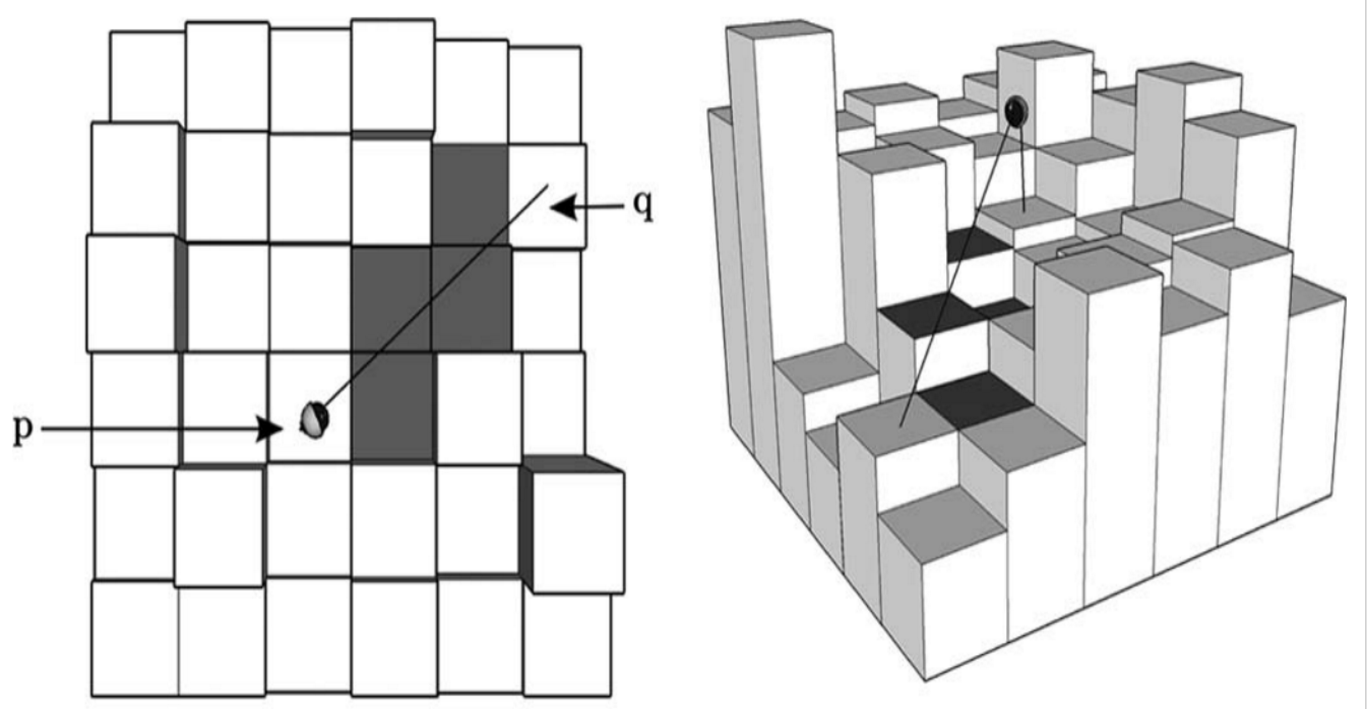
\includegraphics[scale=0.3]{rayTracing.png}
	\caption{An illustration of how ray tracing is used within a 3D environment to identify potential visual obstructions.  Ray tracing is used to determine which cells potentially block the line of sight between the receiver-containing cell $p$ and the target cell $q$.  Shaded cells must be evaluated by a Line of Sight algorithm to determine which portion of the target area in $q$ is visible from $p$. \cite{Akbarzadeh2013}\label{rayTracingImg1}}
\end{figure}

They also present a model for determining Line of Sight based on a gridded 3D system.  Within this system, a 2D grid of elevations represents 3D space as solid rectangular prisms.  The left panel of Figure~\ref{rayTracingImg1} shows how ray tracing is used to determine which cells potentially block the line of sight between the sensor-containing cell $p$ and the target cell $q$.  In the right panel, shaded cells must be evaluated to determine the portion of the target area in $q$ is visible from $p$.


Our simulation is heavily based upon the probabilistic detection models presented by Akbarzadeh et al.  The attenuation, obstruction, and probabilistic detection models are simplified to model omni-directional acoustic receivers.  Because receivers are omni-directional and we assume emplacement a fixed distance off the bottom of the sea floor, we need neither determine the angle of receiver placement, nor the optimal height of receiver placement.  This vastly simplifies our computational complexity, allowing for faster simulation times, and thus iterative designing.


\subsection{Yuan et al - Fast Sensor Placement Algorithms for Fusion-based Target Detection}
The 2008 Yuan et al publication discussed several approaches to maximizing sensor coverage of target areas using the fewest possible sensors.  The defined coverage in terms of the probability of detection $P_d$ and the probability of false positive detections $P_f$.  To be "covered", an area had to have sufficiently high $P_d$ and sufficiently low $P_f$ values.  The team also proposed a probabilistic detection model, where multiple sensors observing the same target could combine their observations via  data fusion to increase $P_d$ and decrease $P_f$ for that target. The model used called for the specification of some number of "target" zones to cover.  The team relied heavily upon a Constrained Simulated Annealing (CSA) algorithm to solve the problem of optimal coverage.  The team found that directly searching for a global optimal solution took exponential time (O(n!)).  The team's second approach utilized a divide and conquer algorithm, which found local solutions for each target area individually, then combined local solutions into a single global solution.  This approach took polynomial time, but resulted in an inefficient global solution.  The authors suggested that, first choosing locations that covered multiple spots, then adding sensors to solve local coverage deficits could improve the algorithm's results.  The final algorithm presented by the team combined a clustering algorithm and the improved divide and conquer strategy.  The clustering algorithm first grouped target locations into larger clusters, then solved for these clusters locally before combining them for a global solution.  This approach both improved the runtime and reduced the total number of required sensors.

The goal of our framework is to recover the greatest number of unique acoustic transmissions given a fixed number of acoustic receivers.  Yuan et al focus on minimizing the number of receivers required to achieve coverage over a given number of target areas.  While their research is very closely related to the goal of our framework, the workflows are fundamentally different.  We believe that SAON designers will more likely find themselves with a finite number of resources to collect as much data as possible (in line with our framework's goal), rather than attempting to achieve specific coverage for target areas.  Still, the ability to address specific coverage requirements is valuable.  Researchers with little knowledge of a target species would likely use our framework, while projects with more refined understandings of their target species would want to utilize Yuan et al's workflow.  


\section{The Economic Value of Information}
\subsection{Hansen \& Jones - The value of Information in Fishery Management}
In their 2008 publication, Hansen \& Jones address the value of information in ecological management through the lens of economic opportunity cost.  In economics, opportunity cost describes the cost of taking a particular action as the value lost by not taking an alternative action.  The authors argue that by investing too heavily in analysis, few resources remain for responsive action.  An underlying assumption is that there is a vast amount of uncertainty in ecology, and that fully realizing the complexities of an ecological system is impossible, no matter how much money is spent attempting to do so.  They also argue that while collecting more information can reduce uncertainty, it is reasonable to assume that there are diminishing returns on the resulting actions (certainty is not linearly correlated with the benefit of the resulting action).  Therefore, they argue that researchers should spend fewer resources on information gathering and more resources on ecological action.  Given fixed research budgets, the opportunity cost of information gathering is then the ecological benefit of action.  

The authors cite two case studies, the first involving the removal of juvenile parasitic sea lampreys from rivers feeding Great Lakes.  Current treatment practices for the project begin by identifying which streams are most in need of treatment, chemically treating those streams, and counting the number of dead juveniles that flow downstream.  The authors note that the cost of analysis (site identification and mortality determination) was nearly a third of the chemical treatment budget.  They argue that by taking an "adaptive" management approach (spending less on data collection and more on treatment), more streams could be treated, leading to a larger ecological impact, despite less accurate assessments.

The second case study was the specification of a global network Marine Protected Areas (MPAs) sufficient to protect the biodiversity and sustainability of fisheries worldwide.  The estimated cost for such a network is between 5 and 19 billion dollars.  The authors claim a mindset exists that MPAs will be more effective if carefully chosen, and that no census exists on where MPAs should be placed. There is little research into correlation of costs for defining MPAs to the effectiveness of the resulting MPA network.  It is believed that a multitude of designs could be "optimal", indicating that suboptimal configurations will result in minimal losses.  The authors claim that all else being equal, spending less on MPA identification, and simply creating more MPAs will reduce the chances of failing to protect a critical location.  Furthermore, the longer it takes to identify MPAs, the more the biodiversity at those sites degrades.  The authors conclude that investments in information gathering should be carefully weighed against other management actions, with the goal of maximizing real-world impacts.

It is important to note that the authors neither excuse nor endorse action without data collection.  Rather, they point out that focusing too many resources on information gathering diminishes ecological impact.  Applying this rationale to our simulation, recreating a perfectly faithful representation of the real world is difficult if not impossible, as there are a great many environmental an physical phenomena that can affect acoustic transmissions.  Modeling all of these phenomena would greatly increase the time and resources necessary to simulate them.  It is important to keep in mind that in practice the framework will likely be used to run several times as researchers tinker with and refine their simulation parameters.  Therefore, an overly complex simulation with a very long run time (hours, days, weeks) could cost many research hours. At the same time, over simplifying a simulation (to the point that it begins omitting significant phenomena) in order to reduce its runtime is a mistake.  If these two "bad" simulations represent the extremes of simulation, then  we contend that a "very good" simulation would consider phenomena that strongly affect the simulation results, and run in a reasonable amount of time.  




\chapter{Design}
\label{design}
\section{Program Requirements}
\label{programRequirements}

\subsection{Motivation}
While the detriments to SAON technologies are well-known \cite{Akbarzadeh2013}, \cite{Heupel2006}, \cite{Howard2002},  \cite{Kessel2015}, \cite{Steel2014} there few tools/services to analytically design SAONs around them.  Further, none of these tools/services are free and open-source.


\subsubsection{Cost Efficiency}
\label{motivationCost}
In section~\ref{CostAltTech}, we discuss the costs of marine telemetry systems, noting that acoustic telemetry systems produce data at a significantly lower ($\ge$10x cheaper) cost than VHF or GPS/Satellite based technologies.  In order to maintain the cost-efficiency of acoustic technology, at least 10$\%$ of the produced transmissions must be captured by the SAON's receiver array.  Given the numerous (but avoidable) impediments to reception of these acoustic signals (\ref{RulesOfThumb}), the array-design process becomes critical to maintaining the cost-efficiency of SAON technologies.  A free network design tool would help to maintain the cost-efficiency of SAONs by eliminating costs surrounding their design and evaluation.  


\subsubsection{Metrics}
\label{motivationMetrics}
The computation of network metrics (Absoloute Recovery Rate, Unique Recovery Rate, Network Sparsity) is very labor intensive at large scale.  Additionally, the process of computation may vary from experiment to experiment.  An automated tool would solve both issues by providing a fast, simple, repeatable, and well-documented method for computation.  Metrics from such a tool would be useful in directly comparing different network deigns.


\subsubsection{Transparency}
\label{motivationTransparency}
An open-sourced tool/service would make the design process more transparent, permitting peer-review and modification.  This would provide increased confidence in the process, and increased adoption of the tool.  Increased adoption would result in a larger number of efficient SAONs, leading to higher data recovery rates, better data quality, increased return-on-investment, and the ability to better address scientific-research questions.


\subsection{Supported Workflows}
\label{workflows}
\subsubsection{Static Analysis}
\label{staticAnalysis}
As mentioned in section~\ref{motivationMetrics}, a primary motive for this tool was the ability to create a repeatable means of measuring the performance of a SAON.  To this end, the ability to measure an existing network design is important.  Users should be presented with network metrics after specifying bathymetry, receiver locations, network properties, and an animal model for a given study site.


\subsubsection{Optimal Design}
\label{optimalDesign}
The primary motive for this tool is the ability to design optimal SAONs.  Users should be presented with a network design (optimal receiver locations), and network metrics after specifying bathymetry, the number of receivers in the network, network properties, and an animal model for a given study site.


\subsubsection{Optimal Addition}
\label{optimalAddition}
Similar to the problem of optimal design, is the problem of optimal addition: the augmentation of an already existing SAON.  Users should be presented with a network design (optimal augmenting receiver locations), and network metrics after specifying bathymetry, the number of receivers to add to the network, network properties, existing receiver locations, and an animal model for a given study site.

\section{Conceptual Model}
\label{conceptualModel}
\subsection{Time/Space Modeling}
\label{timeSpaceModel}
\subsubsection{Spatial Modeling}
\label{spatialModeling}
To model a 4-dimensional underwater environment (a 3-dimensional spatial grid of various attributes), we use a two-dimensional grid of cells (in the x and y dimensions) containing numerical values.  Numerical values in those cells, combined with other user-defined values, can then be used in various shape functions to generate a third dimension (z) of values for that cell.  In this way, we save significant amounts of memory by computing values for a specific three-dimensional cell on the fly, instead of storing an additional dimension of values.  

\subsubsection{Temporal Modeling}
\label{temporalModeling}
With respect to the passage of time, our model assumes that receivers are stationary throughout the entire experiment.  Furthermore, the animal model does not represent animal movement over time, but the percentage of time an animal would spend in a particular cell over the entire study period.  The animal model therefore represents the tendency of an animal's movements over the expected study period rather than its particular movements in a small time period.  As a result, we need not consider temporally-related phenomena. 




\subsection{Bathymetric Modeling}
\label{bathymetyricModeling}
\subsubsection{Bathymetric Grid}
\label{bathymetricGrid}
Bathymetry files are generally given as two-dimensional matrix of numerical values or a list of x,y,z values.  Bathymetric files describe a three-dimensional space as a regular grid of rectangular prisms (cells) with constant length (x-dimension) and width (y-dimension), but varying negative (depth is negative)  heights (z-dimension).  The resolution of a bathymetric file is given by the x and y (length and width) dimensions of its cells.  For example, a 50 meter Bathymetry file has cell sizes of approximately 50 meters square (although these cells are not necessarily perfectly square).  Bathymetric files list beginning and ending coordinates (North/South Latitudes and East/West Longitudes), as well as the grid size (in rows and columns) in cells.  With these two measurements, one can compute the degrees per cell of latitude and longitude.  Thus, particular latitudes and longitudes can be converted to rows/columns, and back.  

Our program works on a two-dimensional, grid-based system, taking advantage of the grid given by the user-provided bathymetric file.  As stated in section~\ref{spatialModeling}, the bathymetric grid is a grid containing numerical values that describe a third dimension (depth).  The exact spatial extent of this description is given by the bathymetric file.  Thus, the resolution of our program's output is dictated by the resolution of the input bathymetric file. 

\subsubsection{Bathymetric Filetypes}
Two highly popular file formats in Geographical Information Systems are provided by NetCDF and ArcGIS.  NetCDF provides an open source file format that lists a header of metadata and a white-space delimited matrix of numerical values.  ArcGIS is a private institution that supplies many different file types, formats, and encodings for a family of GIS-related software systems.  ArcGIS also supports the encoding and transcription of its proprietary formats to the NetCDF format.  Due to the large number of possible format and encoding combinations in ArcGIS file formats and the ability to translate file these various formats to NetCDF, we natively support the NetCDF standard, and assume that users are capable of converting their data into the NetCDF format.  


\subsubsection{Bathymetric Resolution}
Two key components of our program are the animal model and the bathymetric shadowing model.  These models make decisions based upon the depth at a particular cell and the distance between cells, data which is governed by the input bathymetry file.  As stated in Section~\ref{bathymetricGrid}, the resolution of the program's output is dependant upon the resolution of the input bathymetry file.  Obviously, higher resolution grids will offer higher resolution results; but, high-resolution bathymetric files tend to be difficult to come by.  These files are often held by private agencies, or simply never released to the public.  It may then seem useful to artificially increase the resolution of the simulation by dividing the input file's bathymetric cells into sub-cells of finer resolution, but doing so increases the computational size of the program without meaningfully increasing the accuracy of the results.    
 
 
When subdividing cells, either the sub-cells are given the same depth as their parent cell, or the depth of a sub-cell is interpolated from surrounding cells by some smoothing function.  Subdividing a cell into sub-cells with the same depth makes the assumption that all sub-cells are actually the same depth.  Furthermore, this results in the animal and bathymetric shadowing models making the same depth-based decision for all sub-cells that they would for the larger parent cell, increasing the computational load (see Figure~\ref{duplicate}).  Subdividing a cell into sub-cells with a depth governed by a smoothing function makes the assumption that there are no impeding obstacles between neighboring cells, and that there is a smooth transition between them (see figure~\ref{smooth}).  Subdividing the two cells in Figure~\ref{LoS} half (ignoring for now the y component of our grid) results in the four sub-cells with depths given by a smoothing function (Figure~\ref{smooth}) would result in the large depth change at the sheer cliff face in Figure~\ref{LoS} being smoothed into smaller changes in depth, which would allow the unobstructed transmission of acoustic signals.
\begin{figure}[h!]
	\label{resolutionScale}
	\begin{subfigure}[t]{.4\textwidth}
		\centering
		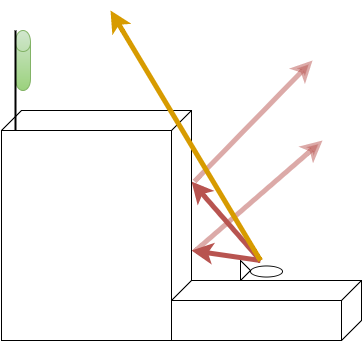
\includegraphics[width=\linewidth]{LoS.png}
		\caption{}\label{LoS}
	\end{subfigure}
	
	\begin{subfigure}[t]{.4\textwidth}
		\centering
		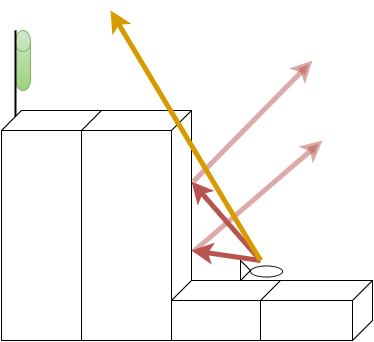
\includegraphics[width=\linewidth]{duplicate.png}
		\caption{}\label{duplicate}
	\end{subfigure}
	
	\begin{subfigure}[t]{.4\textwidth}
		\centering
		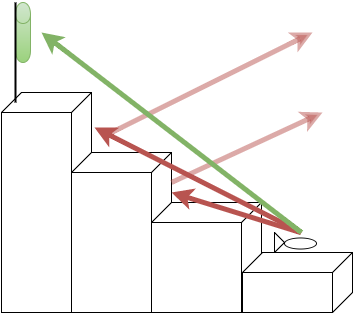
\includegraphics[width=\linewidth]{smooth.png}
		\caption{}\label{smooth}
	\end{subfigure}
	
	\caption{Figure~\ref{LoS} illustrates the bathymetric shadowing model for two adjacent cells within a bathymetric grid.  Figure~\ref{duplicate} shows how artifically increasing the resolution of the bathymetric grid form Figure~\ref{LoS} using the duplication method of cell sub-division does not affect the bathymetric shadowing model.  Figure~\ref{smooth} shows how artificially increasing the resolution using a smoothing function can lead to inflated signal reception.}
\end{figure}

Both strategies (duplicating depth and applying a smoothing function) for artificially increasing the resolution of a bathymetric file disregard the manner in which the bathymetry was originally observed.  Bathymetry is almost always computed as the average observed depth at several points within a geographic area of a given size (resolution).  For example, imagine a particular cell in a bathymetric grid has a steep cliff running across the middle.  Assuming that the sea floor at the top and base of the cliff were perfectly flat, and one measurement was taken at the top of the cliff and one at the bottom, the cell would have a depth equal to the average of the two observed depths.  This average depth would then represent the depth for that entire cell, modeling it as a perfectly flat surface.  Obviously this is problematic as the true nature of the sea floor is misrepresented.  This misrepresentation leads to two conflicting arguments, the first is that the application of smoothing functions or duplicating depths of already averaged data makes faulty assumptions about real-world bathymetry.  On the other hand, because source bathymetric files already represent aggregate data, one could argue that any conclusions drawn from the source bathymetry files are already faulty.  We argue that the conclusions one can make are only as good as the bathymetric information available.  As the resolution of measured bathymetry (bathymetric measurements taken from the real world) increases (becomes finer), so too does the accuracy of the simulation.  While artificially increasing the resolution of a source bathymetric file may skew results, it is sometimes useful for meshing two bathymetric source files of varying resolution into one larger bathymetric dataset.  Our program does not currently support modifying the resolution of source bathymetric files.


\subsubsection{Bathymetric Shadowing}
\label{bathymetricShadowing}
In the real world, the transmission of an acoustic ping originates from the tagged animal and propagates to the receiver.  This propagation is governed by complex interactions with the surrounding environment (including the bottom substrate, water density, distance to the surface/sea-floor, thermoclines, the number of tagged animals in the vicinity, and ambient noise).  Because it is difficult to model these phenomena without significant data on a large number of variables over a large area, our simulation uses a simplified propagation model relying on direct line of sight between a tagged animal and a receiver.  Simply put, in order to receive a transmission, there must exist a physically-unobstructed path between a tagged animal and a receiver.  


\subsection{Animal Modeling}
\label{animalModeling}

\subsubsection{Behavior Grid}
\label{behaviorGrid}
Animals exhibit many different movement patterns and habitat preferences (both of which can vary in three-dimensional space).  This greatly affects their distribution within the study space, and thus the network configuration that should be deployed to capture their movement.  To describe the distribution of transmissions released from tagged animals, we utilize a two dimensional grid of the same dimensions and resolution as the Bathymetry Grid (Section~\ref{bathymetricGrid}).  Each cell in this "Behavior Grid" contains a positive real value indicating, out of all transmissions that will be released over the entire experiment period, the percentage of transmissions that are expected to be released from within that cell's water column.  This value can loosely be though of as the "animal-residency" of a cell since we are effectively measuring the number of animal-hours spent in that cell.  

To populate this 2D grid with values, we provide two behavioral models to simulate the horizontal distribution of animals, and two optional models for the vertical distribution.  Note: we use the terms "animal" and "transmission" interchangeably as we are interested in capturing acoustic transmissions, which are given off by the tags carried by the target species.  


\subsubsection{Animal Movement Modeling}
\label{animalMovementModel}
To simulate tagged animal movement across the two dimensional x/y space (as one would expect to see on a map from above), we provide two basic probabilistic movement models: Random Walk, and Ornstein-Uhlenbeck(OU).  

\paragraph{Random Walk Model}
\label{randomWalkModel}
The Random Walk model assumes that animals move randomly through the environment.  As a result, over the entire study period, each valid grid cell (as defined by the Restricted Vertical Habitat Range (Section~\ref{restrictedVerticalHabitat})) will see an equal amount of animal traffic.  The result is that every valid cell  in the grid will have the same chance of capturing an animal's acoustic transmission.  We assume that tagged individuals will be willing and able to very briefly (in probabilistically negligible time frames) pass through inhospitable (over dry land, through impassible terrain) cells to get to other cells.  This means that disjoint sections of habitat are still equally likely to see animal presence.

\paragraph{Ornstein-Uhlenbeck Model}
\label{ouModel}
The Ornstein-Uhlenbeck(OU) model\cite{OU} supports the idea that over time, animals will tend to congregate near certain points of interest.  This concept models an animal's desire to seek out and remain near a physically significant structure, a region of high food availability, breeding grounds, shelter, etc.  The OU algorithm allows for the modeling of the attraction towards a focal point in the x/y directions separately.  Assuming a center point at the origin of a Cartesian grid, increasing the attraction in the x-direction will bring the distribution closer to the x-axis, and decreasing it will spread the distribution away from the x-axis.  A correlation value ($-1\le x \le 1$) allows for tilting the angle of the distribution.  A positive correlation value tilts the distribution clockwise, and a negative correlation value tilts it counter clockwise.  Correlations of 0 (no tilt), 1 ($180^{\circ}$ tilt), and -1 (-$180^{\circ}$ tilt) will have no observable effect on the distribution.
\begin{figure}[b]
	\label{OUimg}
	\centering
	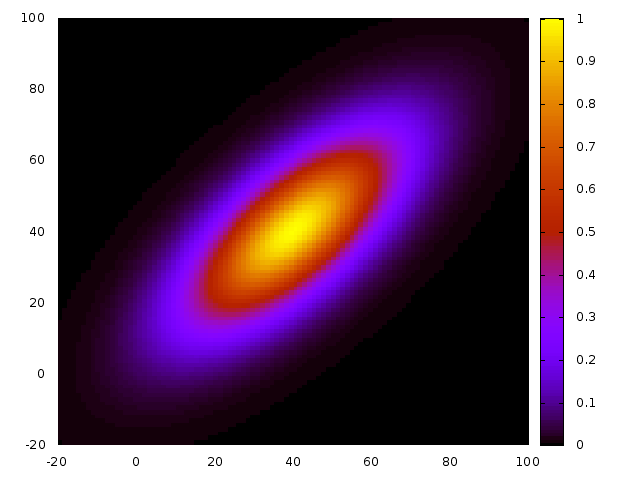
\includegraphics[scale=0.5]{OUpos7.png}
	\caption{}\label{ouimg}
	\caption{An example of a distribution given by the Ornstein-Uhlenbeck Model with a high attraction value in the x-direction, a low attraction value in the y-direction, and a correlation value of 0.7.}
\end{figure}


\subsubsection{Habitat Preference}
\label{habitatPref}
Some animals exhibit the preference to reside within a specific section of the water column; for example, prey animals may prefer hiding in reef heads at the bottom of the water column, while predators will prefer to hover several meters off the bottom.  This preference can be incorporated into the animal model by specifying mean (preferred Depth") and standard deviation("SD of Preferred Depth") values.  These values are given as a measure of the distance (in meters) from the bottom.  For example, specifying a depth of '0' for Preferred Depth indicates that the animal prefers to live on the sea floor, while a value of '5' indicates that the animal prefers to live 5m off the sea floor.  Allowing a standard deviation value allows for the modeling of animals that tend to be sedentary within the water column (a small deviation), and those that migrate through the water column (a large deviation).  Currently, the simulation does not support the modeling of sub-surface animals, and any part of the distribution curve falling below the sea floor will be redistributed along the rest of the curve. 


\subsubsection{Restricted Vertical Habitat Range}
\label{restrictedVerticalHabitat}
Some animals will live only in a specific depth range.  For example, a deep sea fish may live only in depths of 300-400 meters.  To incorporate this into the behavioral model, users can specify a minimum and maximum vertical habitat range for their animal.  If this option is selected, the program will only simulate animals in cells whose maximum depths are between the given minimum and maximum depths.  As in the Random Walk Model, we assume that animals are willing and able to move between disjoint areas of habitat.


\subsection{Receiver Modeling}
\label{receiverModel}

\subsubsection{Acoustic Attenuation}
\label{acousticAttenuation}
As acoustic transmissions travel away from their point of origin, they experience significant attenuation.  We model this attenuation of acoustic signal as a deteriorating function following a Gaussian distribution.  Given a particular distance between a tag and receiver, this distribution describes the probability of capturing the transmission.  Depending upon the environment, the highest probability of detection generally occurs a few meters away from the receiver.

\subsubsection{Detection Range}
\label{detectionRange}
The distance at which a transmission from an acoustic tag can be captured is largely determined by the transmission power of the acoustic tag.  In our model, we assume that all animals have the same model of acoustic tag, and that "transmission range" is instead a property of the receiver referred to as "detection range" ($D_{range}$).  We define the detection range of a receiver to be the average distance (specific to the given study site) at which the probability of detection drops to 5\%.

\subsubsection{Detection Area}
We define the Detection Area of a receiver to be the square plane of grid cells around a receiver which will be considered when evaluating a potential receiver emplacement.  Theoretically, the Detection Area of a receiver is a circle with a radius equal to the receiver's detection range ($D_{range}$).  Within our program, we model the Detection Area as a square grid of cells with an edge length equal to 2*$D_{range}$ + 1, centered on the cell where a receiver will theoretically be placed.  The additional cell ensures odd dimensions for the square, so that there exists a central cell to model as the receiver.  We model a square instead of a circle for simplicity of book keeping (we simply keep track of the detection range, and starting row/column indexes).  The theoretical Detection Range can then be imagined as a circle circumscribed in the square of our model.  At first glance, it might seem that this simplification would alter the probabilistic distribution models as additional "gray" cells (those outside the circle but within the square) are being considered.  However, this is not the case as those models utilize exponential functions based on the absolute distance from the receiver.  Gray cells will therefore contribute exponentially less to the total probability than those cells within the detection range, and their effect on the final probability will be negligible.  

\subsubsection{Network Specification}
There are three distinct ways to place receivers into the model: user specification, optimal placement, and optimal projection.  User Specified Receivers (USR) represent receivers that are already deployed at the study site and are being integrated into a larger network.    Program Placed Receivers are receivers that will be  optimally placed by the program, taking into account existing (user specified) receivers placements using the suppression dynamic explained in section~\ref{suppression}.  Projected Sensors are PPSs that do not count towards the network statistic rates returned by the program.  Instead, their contributed recovery rates are given separately, and represent the marginal benefits of incrementally placing more receivers.  


\section{Evaluation Algorithms}
\label{evaluationAlgorithms}

\subsection{Evaluation of Receiver Emplacements} TODO needs work
\label{evaluationOfReceiver}
Section~\ref{animalModeling} discusses the models used to simulate animal movement.  The animal movement models provide the "Behavior Grid", a 2D grid (of the same size as the specified bathymetry grid) which gives the distribution of animals across the study area, and a shape function which describes a normal distribution of animals within the water column at various depths.  Section~\ref{LoS} discusses the Line of Sight (LoS) model used to simulate the obstruction of acoustic transmission.  Section\ref{receiverModel} discusses how attenuation affects the propagation of acoustic signals and thus the probability of detecting ($P_{range}$) acoustic transmissions from a distance.

\subsection{Evaluation Algorithms (Bias)}
The Evaluation or “Goodness” algorithm is the driving force behind the evaluation of sensor placements.  Given a particular cell at row i and column j, an Evaluation Algorithm will compute a non-negative, rational value representing how well cell (i,j) conforms to that Algorithm's definition of "good".  These values are computed for all cells within the Bathymetry Grid, and stored in the Goodness Grid, a 2D grid of identical size and resolution as the Bathymetry and Behavior Grids.  Thus, $G_{i,j}$ refers to the goodness value of the cell at row i, column j on the bathymetry grid.  

While users are able to write their own “Goodness” algorithms, three basic algorithms are provided.  All Evaluation Algorithms compute the goodness of a potential receiver location ($G_{i,j}$) by summing the number of Estimated Receivable Transmissions (ERT) from all cells within Detection Range of $G_{i,j}$.  The various options each compute ERT differently.

\subsubsection{Animal Only (Option “1”)}
This option prefers to place sensors in areas of high animal activity, completely oblivious to the surrounding bathymetry.  This is useful for when no bathymetric information is available or when animal activity occurs well above the sea floor.   The "Animal Only" option computes ERT for a cell as the animal-residency of a cell (according to the Behavior Grid), multiplied by the probability of detection due to attenuation for that cell's distance from the receiver.


\subsubsection{Visible Fish (Option “3”)}
This option chooses sensor locations that have the best view of areas of high animal activity.  Both animal presence and visibility due to topography are considered. TODO


\subsubsection{Topography Only (Option “2”)}
This option places sensors in areas that have the best visibility of the surrounding area, regardless of the expected animal-residency.  This is useful for experiments where animal habitat is unknown or to be determined.  Here, ERT is computed as the number of observable transmissions from a uniformly distributed animal model.  While this algorithm is referred to as "Topography Only", we implement this by using the "Visible Fish" algorithm with a simplified animal model.  Specifically, we assume that animals are uniformly distributed throughout the environment.  Because animals are uniformly distributed, the more volume a receiver can see, the more transmissions it will receive.  Thus, the algorithm will value cells with the best possible view of the surrounding water columns.



\subsection{Computational Complexity}
\label{computationalComplexity}
A naive solution might be to determine whether or not each cell in the three-dimensional grid can see the receiver.  Given that the volume of a sphere is $\frac{4/3}\pi r^{3}$, this solution would need to consider O($r^{3}$) cells.  Recall however, that we are using a 2-dimensional grid as the basis of our simulation and computing the third dimension as necessary by using a shape function.  Therefore, it is much more computationally efficient to determine the deepest depth in each cell that can be seen by the receiver, and then use integration to compute the probability of detecting transmissions within the water column above that cell ($P_{d}$) .  This leads us to the problem of finding the greatest depth (in each 2D cell) which is visible from the receiver.  We quickly compute this via incremental ray tracing which can be done in O(1) time for O($r^{2}$) cells \cite{Akbarzadeh2013}.   Then, using integration over the shape function, and known min/max depths, the total ($P_{d}$) can be computed in O($r^{2}$) time.  Finally, we determine an average($P_{d}$)  over all O($r^{2}$) cells within detection range.  This metric is used to evaluate each cell within the study area as a candidate for receiver placement.  Thus, our method for evaluating a 3D space can be done in  O($r^{2}$ + $r^{2}$ + $r^{2}$) = O($r^{2}$) time.  One notable difference between our method and the naive method is that the naive method computes the sum probability of detection for each cell in the 3D space, where our method simply integrates to find the probability of detection for the entire a column of water.  


\begin{figure}[t]
	\label{rayTracing}
	\centering
	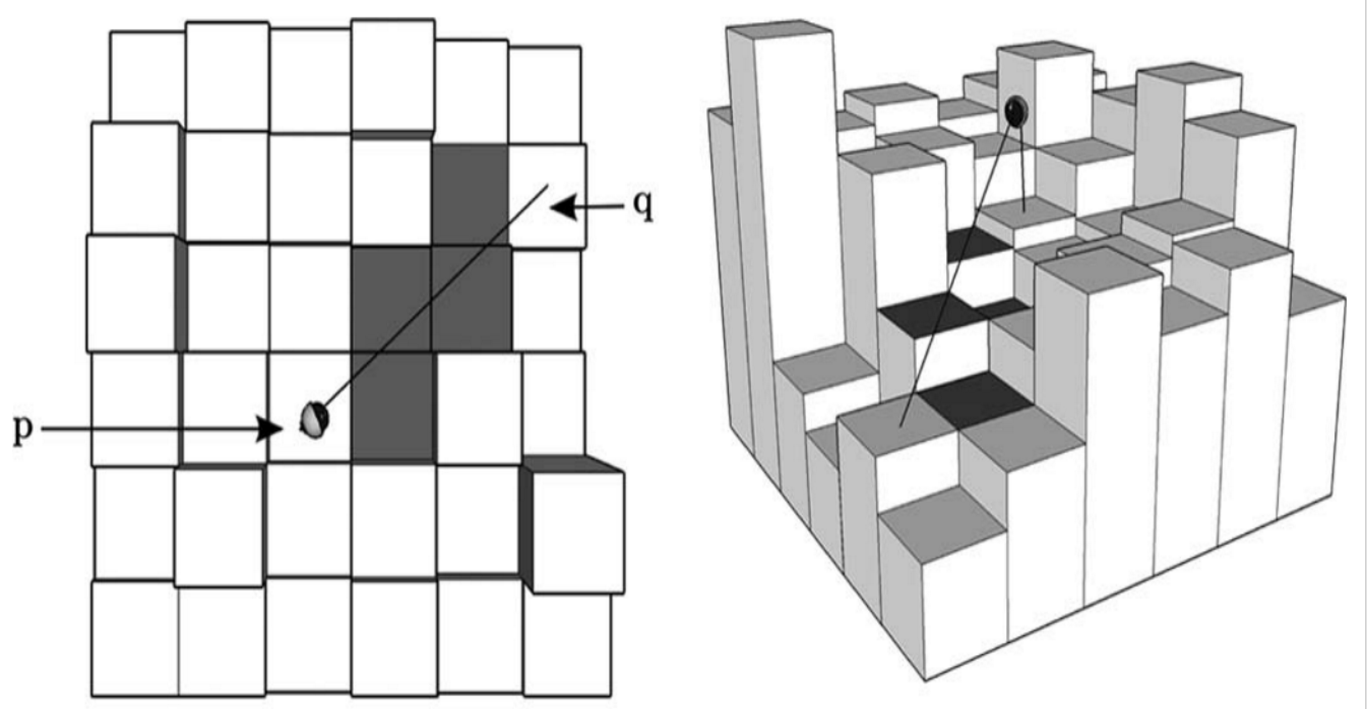
\includegraphics[scale=0.3]{rayTracing.png}
	\caption{An illustration of how ray tracing works within a 3D environment. \cite{Akbarzadeh2013}}
\end{figure}

\begin{figure}[t]
	\label{observableAnimals}
	\centering
	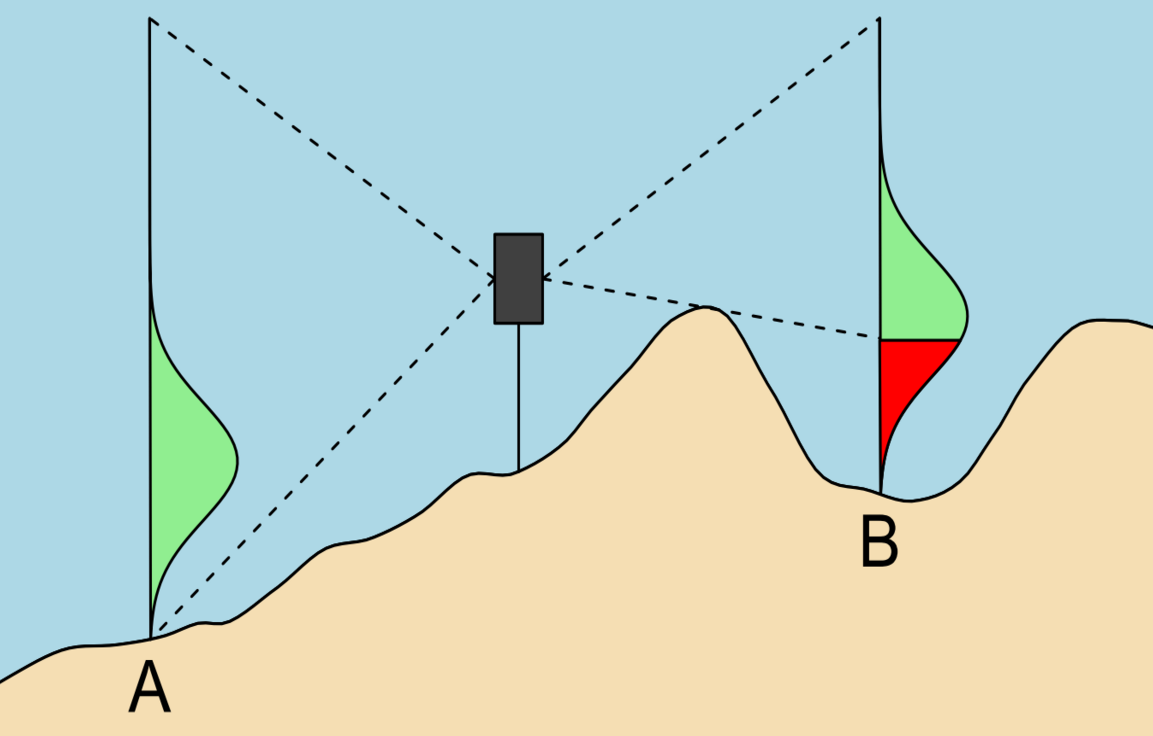
\includegraphics[scale=0.3]{ObservableAnimals.png}
	\caption{An illustration of how ray tracing and integration over a shape function can be used to compute the probability of detecting fish within a cell.  Dotted lines indicate the maximum and minimum depths visible to the receiver.  The normal distributions in green/red indicate the distribution of fish within a given cell as determined by a shape function.  The green portion of the distribution indicates the portion of the distribution that is observable by the receiver and the red indicates the portion that is unobservable by the receiver.  The observable distribution (green) is computed by integration over the shape function.}
\end{figure}


\subsection{Selection of Optimal Emplacements}
\label{selectionOfOptimalEmplacements}
Section~\ref{evaluatingSensorEmplacements} describes the evaluation of cells as potential receiver locations.  The Optimal Design and Optimal Addition work flows (section~\ref{workflows}) require the identification and selection of a user-specified number of receiver emplacements.  Once all cells within the area of interest have been evaluated, the program simply selects the highest rated cells.  The program first selects the user-specified number of optimal receiver locations, and then the number of specified projected receivers.


\section{Suppression}
\label{suppression}
As previously mentioned, the optimality of a network depends greatly upon the way in which data quality is defined.  Some users will want to design a network that covers as much of a study area as possible, while others might want to heavily saturate a small area with sensors to facilitate higher resolution data.  Others may wish to find the receiver locations that return the highest number of unique data points.  Also previously mentioned was the metric of Unique Data Recovery Rate (UDRR) and Absoloute Data Recovery Rate (ADRR) [Section~\ref{dataRecoveryRate}].  For studies which wish to maximize their UDRR, we provide an optional suppression mechanic, which promotes the selection of receiver placements that have a high number of unobserved transmissions.

\subsection{Suppression Area}
As an input to the program, users can specify a Suppression Range Factor as a positive real number.  This factor is used to scale the Detection Range (Section~\ref{detection Range}) and define a grid similar to the Detection Area (Section~\ref{detectionArea}).  The resulting grid is referred to as the Suppression Area.  The Suppression Area is centered over a receiver placement and cells within this area have their number of undetected transmissions reduced according to a Suppression Algorithm.  The suppression mechanic is used during the selection phase of the program.  After selecting each optimal receiver location (Section~\ref{selectionOfOptimalEmplacements}), the Suppression Area around that receiver location is suppressed.  This means that emplacement selection is a sequential process, where selecting each emplacement depends upon the previous selection.  

\subsection{Suppression Algorithms}
\label{suppressionAlgorithms}
To promote the flexibility of our program, we provide users two algorithms for suppression.  The first offers a lower computation time at the cost of divergence from our theoretical model.  The second offers a higher fidelity model, but requires significantly more computation.

\subsubsection{Static Suppression}
\label{staticSuppression}
The Static Suppression algorithm takes a "cookie-cutter" approach and reduces the number of undetected transmissions in the Suppression Area by a user-specified factor.  All cells within the Suppression Area are multiplied by a user-specified value.  This computation is very simplistic, requiring only a scalar multiplication, and as such runs very quickly.  This is useful for simulations that intend to place a very large number of receivers.  The cost of this speed is that the algorithm ignores the attenuation and line of sight models completely.  For instance, a cell that is very far away from the receiver, and whose line of sight to the receiver is obstructed will be reduced by the same factor as a cell with unobstructed line of sight, near the receiver.  Obviously this is not a faithful representation of the conceptual models discussed earlier, but supplied for the sake of convenience.

\subsubsection{Exact Suppression}
\label{exactSuppression}
Let $C_{i,j}$ denote the cell at the $i^{th}$ row and $j^{th}$ column of the 
The Exact Suppression algorithm follows the conceptual model very closely, utilizing the attenuation, and line of sight models via the "Visible Fish" evaluation algorithm (Section~\ref{evaluationAlgorithms}, Bias 3).  The primary purpose of this algorithm was to discount exactly those transmissions which are likely to be observed by a placed receiver.  This algorithm utilizes Algorithm 3, "Visible Fish", to compute the ERT for each cell $C_{i,j}$ within the Suppression Area of the placed receiver $L$.  Then, each cell in the Behavior Grid, $B_{i,j}$  that corresponds to 

Add new receivers (with optimal placement) to an already existing network
Analyze the data recovery rate for a receiver network
Create an optimal receiver network
TODO

\section{Optimal Sensor Projection}
In normal research situations, users will have a set number of receivers to place within their study site.  The process of arriving at this number is likely unscientific, perhaps relying on user estimate (such as the user-perceived feasibility of receiving a given number of receivers).  Rather than guessing at the number of receivers to use, and hoping for an adequate data recovery rate, users should be able to calculate the marginal benefit (additional detections, increased Data Recovery Rates) of utilizing a variable number of receivers.   To this end, the program allows for the projected incremental benefit for a given number of additional receivers.  Our program facilitates this by allowing users to specify a number of receivers to project, returning graphs and metrics of the marginal increase in Data Recovery Rate.  Armed with this data, users can determine an appropriate number of receivers to purchase, or construct an argument for purchasing more receivers.




\chapter{Results}
\section{Output Files}
Our program outputs 6 files:\newline
1) The Bathymetry Grid as a heat map\newline
2) The Behavior Grid as a heat map\newline
3) The Goodness Grid as a heat map\newline
4) The Coverage Grid as a heat map\newline
5) The marginal gain in Unique Recovery Rate as a function of the number of receivers placed\newline
6) Text representations of the 5 Grid files, tabular receiver data, and the specified input parameters.\newline

\subsection{Grid Graphs}
The four Grid files (Bathymetry, Behavior, Coverage, and Goodness) are visualized as a heat maps.  All of these are overlaid with the resulting receiver locations as numbered circles.  Receiver locations show their detection range as dotted circles centered over the receiver locations.  User placed receivers are colored gray, receivers placed optimally by the system are colored blue, and projected receivers (also placed by the system) are colored green.  The numbering on receivers denotes the rank of each receiver's Unique Data Recovery Rate.  User and system-placed receivers are ranked separately.  The highest ranked system-placed receiver locations are returned as the optimal receiver locations, with the lower ranked locations as the projected receiver locations.


\subsection{Data Recovery Graphs}
The program also produces a graph of the marginal increase in and cumulative sum of the Unique Data Recovery Rate as a function of the number of optimally placed receivers used (Figure~\ref{recoveryGraph}).  The graph of the marginal increase in UDRR (the lower graph) is especially useful.  Given that Receivers have a fixed per-unit cost, it makes sense to weigh a receiver's effectiveness (in this case, UDRR contribution) against its cost to determine the utility of purchasing an additional receiver.  The graph of cumulative UDRR is useful to quickly identify the number of receivers necessary to reach a goal UDRR.

\begin{figure}[ht]
	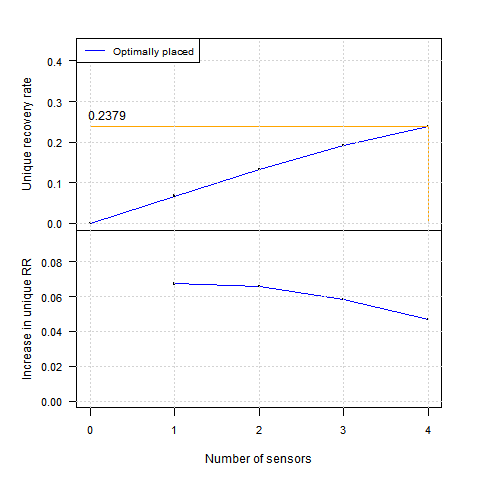
\includegraphics[scale=.7]{RecoveryRates.png}
	\caption{\label{recoveryGraph} A graphical representation of the cumulative and per-receiver UDRR.  User-placed receivers are representd by a grey line, system-placed receivers are represented by the black line, and projected receivers are represented by the green line.} 
\end{figure}

\subsection{Text Files}
The program returns a comprehensive text representation of the program output (text dump of gridded data and input parameters), and a short, human-readable document that lists the primary simulation parameters (Evaluation Algorithm, Suppression Algorithm, Behavioral Model, Input Grid Size, and Detection Range), as well as a tabular output of receiver placements (coordinates), data recovery rates for each receiver, and network sparsity.  Projected receivers are excluded from the total UDRR, ADRR, and sparsity values.

Coordinates are returned in both a Global (with respect to the original Topography file) and local (the user specified area of interest) frame.  While the curvature of the earth is well documented, different bathymetric maps may handle the mapping of a 3D curved plane to a 2D Grid differently.  For example, one Grid may implement some scaling on Grid cells a function of the cell's latitude or distance from a certain point.  Other Grid files may simply provide non-square Grid files.  By proving a small-scale (local) and large-scale (global) frame of reference for our receiver locations, irregularities of this nature are more easily detected.

\begin{figure}[ht]
	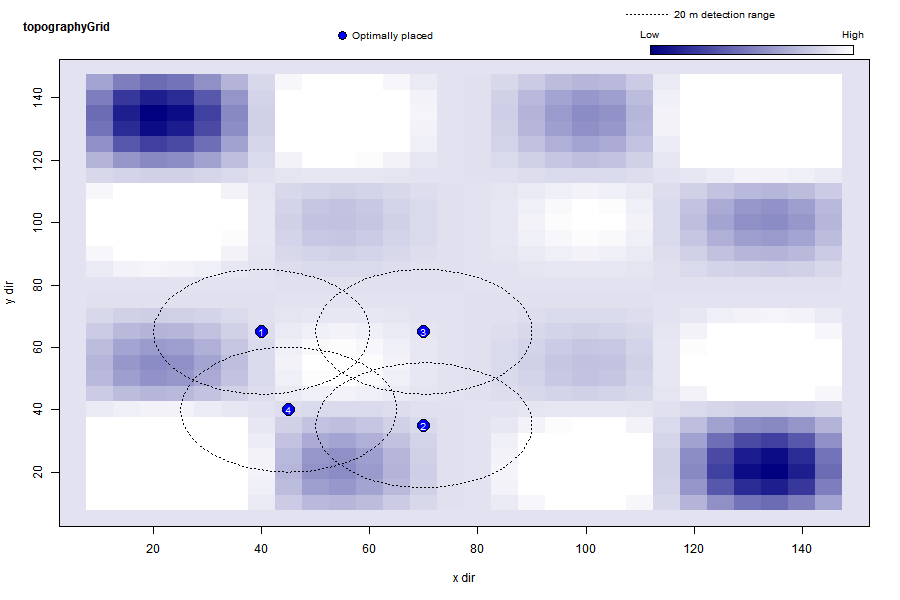
\includegraphics[scale=.5]{TopographyGrid.png}
	\caption{A graphical representation of an artificial Bathymetry file at a 1m resolution (each cell has an edge length of 1m).  Darker cells represent greater depths, while white cells represent inaccessible terrain (dry land).  The optimal receiver locations are shown on the Grid as blue numbered circles, user-placed sensors as grey circles, and projected receivers as green circles.  All receivers have their Detection Range shown as dotted lines.\label{bathyGraph}}
\end{figure}

\begin{figure}[ht]
	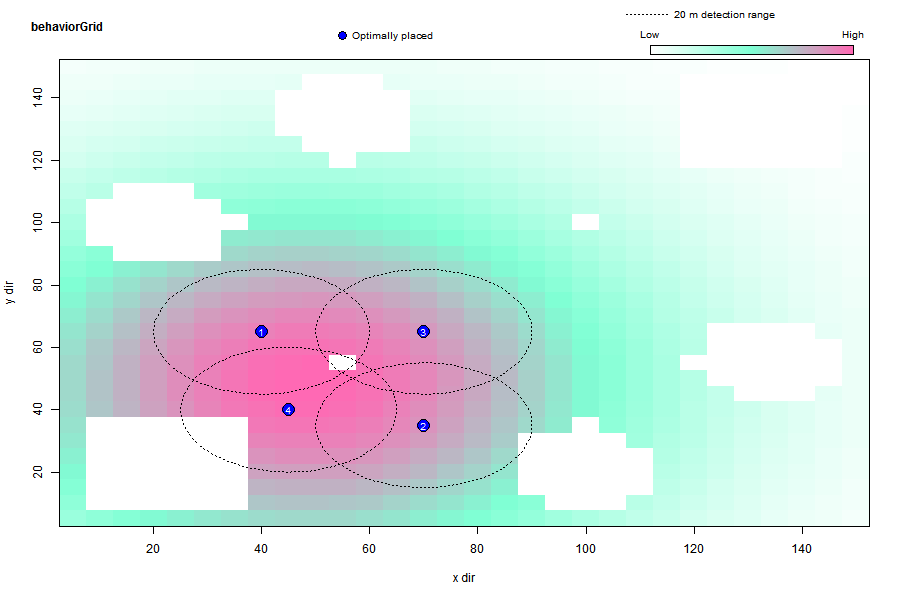
\includegraphics[scale=.5]{BehaviorGrid.png}
	\caption{The Behavior Grid represented as a heat map  Higher levels of animal residency correspond with pink cells, moderate levels as light blue, and white for non-residency (inhospitable habitat such as  dry land).  The optimal receiver locations are shown on the Grid as blue numbered circles, user-placed sensors as grey circles, and projected receivers as green circles.  All receivers have their Detection Range shown as dotted lines.\label{animalGraph}}
\end{figure}

\begin{figure}[ht]
	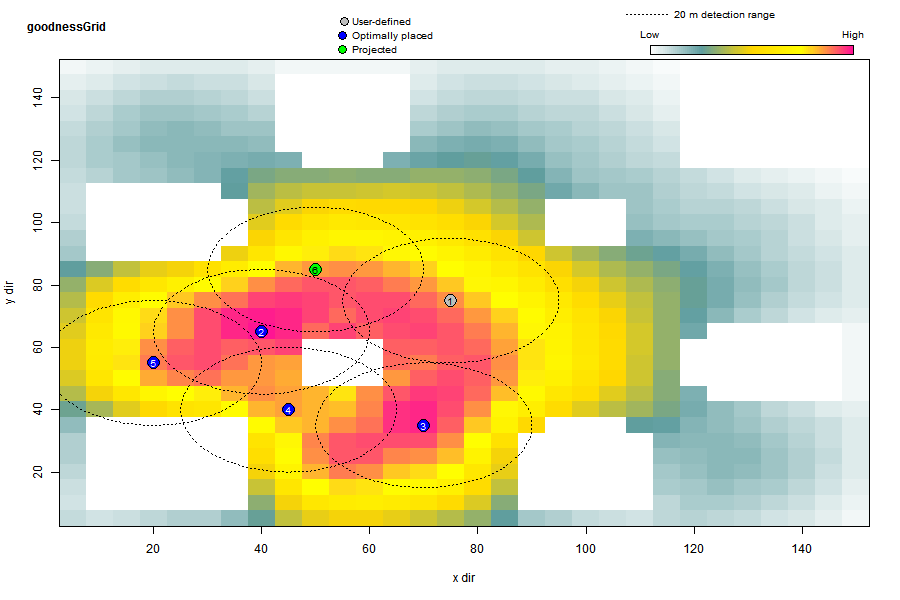
\includegraphics[scale=.5]{GoodnessGrid.png}
	\caption{The Goodness Grid represented as a heat map showing the sum total of Estimated Receivable Transmissions (ERT) for a receiver placed in a particular cell.  The legend in the top right assigns color coding to various ERT values. The optimal receiver locations are shown on the Grid as blue numbered circles, user-placed sensors as grey circles, and projected receivers as green circles.  All receivers have their Detection Range shown as dotted lines.\label{GoodnessGraph}} 
\end{figure}

\begin{figure}[ht]
	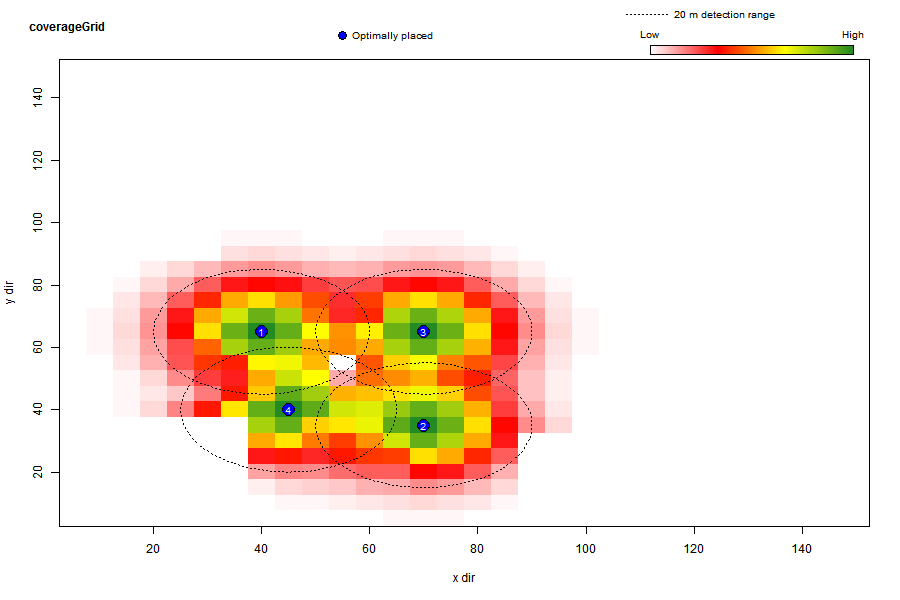
\includegraphics[scale=.5]{CoverageGrid.png}
	\caption{The Coverage Grid represented as a heatmap showing the quantity of Estimated Receivable Transmissions from each cell in the study site, for the designated receiver array configuration.  The legend in the top right assigns color coding to various ERT values.  The optimal receiver locations are shown on the Grid as blue numbered circles, user-placed sensors as grey circles, and projected receivers as green circles.  All receivers have their Detection Range shown as dotted lines.  The missing corner of of Receiver 4's Detection Area is due to the presence of an obscuring section of Bathymetry (dry land).\label{coverageGraph}}
\end{figure}

\section{Nature of Results}
The challenge of acoustic network design is one that is common within the acoustic tracking community, yet rarely addressed.  While there are many methodologies, applications, and services that focus on achieving various objectives, this framework distinguishes itself in its availability, transparency, and adaptability.  

As previously stated, our framework is freely available \cite{acousitcdeploy} and falls under the GNU General Public License (GPL 2).  This availability means our methodologies are fully transparent, and are available for peer-review.  Furthermore, our application is accessible to researchers with and without expertise in R.  We provide a useful set of default options in with a user-friendly interface for users less experienced R developers, and ample documentation for those users with expertise in R.  The modularity of our framework allows R-savvy researchers to adapt the framework to their specific needs.  While other applications and methodologies optimize for fixed-objective functions (k-neighbor coverage, fixed detection probability, etc), our framework allows for user-customized objective functions.

\subsection{Advantages}
The primary advantage of our framework is its flexibility.  Many key functionalities of our framework (Evaluation Algorithms, Suppression, Animal Modeling, Network Statistics) operate over very simple data containers (Grids).   

* Framework = flexible, extensible
* more of a "library" than an application.
* input your own grids

\subsection{Disadvantages}
* using it as a library requires substantial programming ability.
* the default application is quite slow (exhaustive search)
* written in R (slow, brittle)

\section{Future Work}
\subsection{Emperical Analysis}
The analytical framework described herein is largely theoretical, despite a basis in well documented physical phenomena.  In order to better understand the correctness of our analysis, it would be useful to analyze empirical data from small-scale acoustic networks designed with this application.  Specifically, we are interested in the accuracy of our network coverage projections, and the affect of bathymetric resolution on this coverage.  

\subsubsection{Acoustic Coverage}
Recall that estimated data recovery rates are calculated based upon acoustic coverage and animal distribution.  While we provide basic Animal Models, the accuracy of these models (and as a result the accuracy of our data recovery rates) is very species-dependent and outside the scope of this paper.  While data recovery rates are based on animal models, our acoustic coverage model is not.  Thus, we are very interested in the accuracy and optimality of our bathymetric shadowing and network coverage models.  It would be interesting to compare the acoustic coverage of a real-world network designed by our application against our theoretical coverage of that same network.

\subsubsection{Bathymetric Resolution}
Section~\ref{bathymetyricModeling} describes the nature of artificially increasing bathymetric resolution.  It would be interesting to see how varying the native resolution of bathymetry affects the acoustic coverage of network topology both within our framework and in the real world.

\subsubsection{Workflows}
The workflows described in Section~\ref{workflows} were based upon both personal experience and imagined use.  It would be good to investigate the actual use cases, workflows, and problems that researchers face at various points throughout the lifetime of an acoustic tracking project.  By identifying unconsidered problems and workflows, the framework can be modified/expanded to encompass new roles and features, leading to greater usefulness.

\subsection{Heuristic Algorithms}
Recall that the function of the Goodness Grid is to store Goodness values for various locations within the study area.  The sample application simply computes every possible goodness value in the Goodness Grid, and then finds the top values Goodness values via R's $max()$ function.  While this process is guaranteed to find optimal receiver positions, it is computationally intensive, accounting for the vast majority of the program's run time.  Utilizing heuristic algorithms can significantly reduce the number of Goodness values that are computed, but can also reduce the optimality of the final acoustic array.  Heuristics are currently not included in the framework because functions involving Evaluation Algorithms and any new heuristic algorithms will likely be tightly coupled (a heuristic algorithm will likely need to consider an Evaluation Algorithm's definition of $Goodness$).  Furthermore, to avoid computational overhead (such as passing large lists of heuristic candidate cells), it is likely that the heuristic algorithm and Evaluation Algorithm will be called from within the same function.  This will likely lead to a large number of customized functions that implement heuristic algorithm-Evaluation Algorithms combinations.  It would be very useful to evaluate the cost of programatically de-coupling Evaluation and heuristic algorithms and passing large lists of heuristic candidates.  This data could then be compared against the measured benefits of various heuristic algorithms to evaluate the best methodology for integrating heuristics into the framework.  Another useful avenue would be the investigation of Evaluation Algorithm agnostic heuristics, which could provide better run times without tight couplings.

\subsection{Interactive Visualizations}
It could be useful to allow users to interact with the output graphs as a graphical user interface.  Users would able to move receivers around the graph and see how new placements affects network statistics in real-time.  Given that the Goodness Grid can be pre-computed, moving receivers and updating the effects of that movement in real-time requires very little re-computation.  In this case, it might be unnecessary to even pre-compute the Goodness Grid, but instead only preform the Evaluation Algorithm on cells where a user places a sensor.  This would allow users to quickly see how various receiver arrangements affect their network design, and facilitate rapid, impromptu prototyping of various configurations.  

Utilizing 3D visualizations could further enhance the user's understanding of network topology.  Figure~\ref{3d} illustrates a first-person view of the 3D environment modeled by the program.  Here, bathymetry is rendered as 3D mounds, with animal distributions represented by green fish, and receiver coverage by red spheres.  Users might be able to ''swim'' through the 3D environment, viewing their network from various angles.  Such a visualization would help users better understand what is being modeled, how their array is laid out, and where modifications might be helpful.

\begin{figure}[ht]
	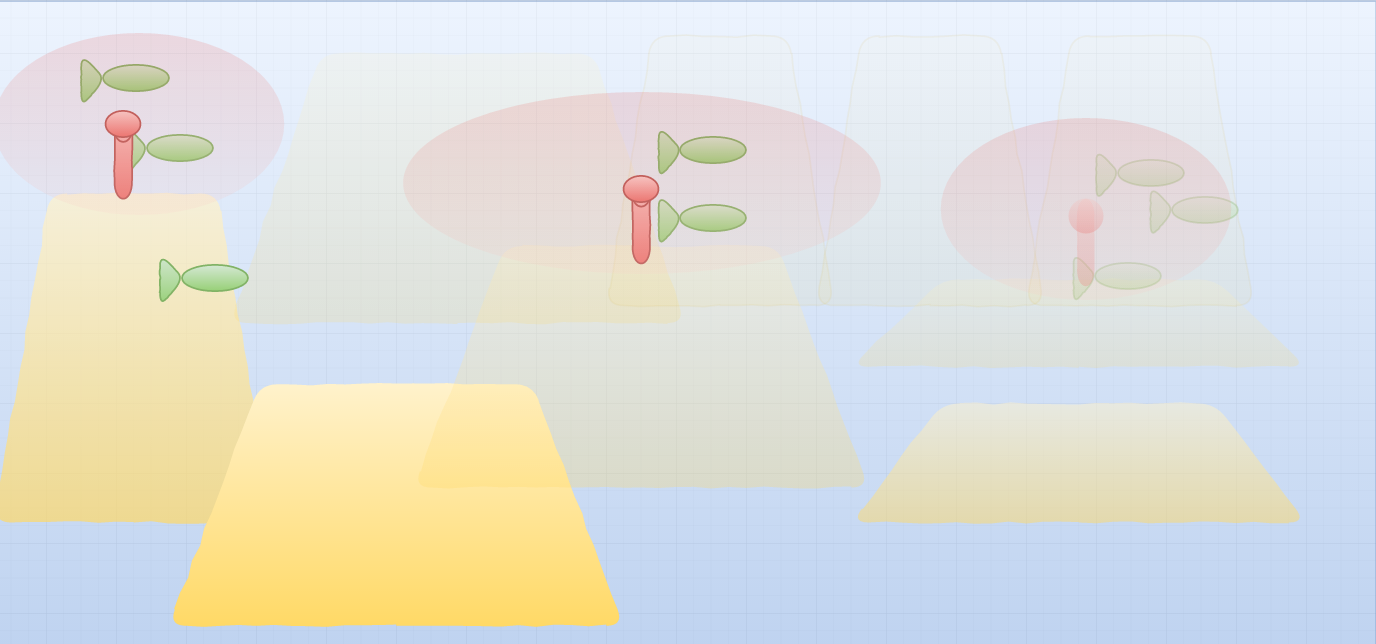
\includegraphics[scale=.45]{3d.png}
	\caption{A first-person view of the 3D space modeled in the program.  Users would be able to ''swim'' through the environment and gain a better perspective on what they are modelling, what their receiver array might look like in the environment, and where more receivers might be needed.\label{3d}}
\end{figure}

\chapter{Conclusions}
We have presented a framework for the optimization and measurement of Static Acoustic Observation Networks (SAONs), the benefits of which are decreased cost of data collection, increased volume of collected data, and higher data quality.  While these benefits are largely realized early on during the design of a SAON, the framework's utility extends into the augmentation and assessment of acoustic tracking studies.  The ability to include an already existing SAON in the design process allows for the optimal augmentation and integration of SAONs.  This is useful to projects that operate on annual budgetary allotments and periodically purchase and deploy of hardware.  By supporting this incremental growth pattern, our framework can be used to make optimal use of limited resources.  This functionality also provides a mechanism for researchers from separate studies to pool resources, mesh disjoint networks, and collaboratively increase data recovery rates.  Our also framework provides automated metrics for the evaluation and comparison of SAONs.  These metrics facilitate the evaluation of existing and theoretical network topologies, which is useful when demonstrating the need for additional hardware.

Our framework is customizable, allowing users to develop their own Behavior, Evaluation, and Suppression Algorithms, Shape Functions, and metrics.  Coupled with the fact that our program is open source (the source code is freely available and editable \cite{acousitcdeploy}), and free to use, we expect this tool will have a strong impact on the acoustic tracking communities.  


%%% Switch to appendix mode
\appendix

%%% Bring in any appendices from external file (optional)
%%%%%%%%%%%%%%%%%%%%%%%%%%%%%% -*- Mode: Latex -*- %%%%%%%%%%%%%%%%%%%%%%%%%%%%
%% uhtest-appendix.tex -- 
%% Author          : Robert Brewer
%% Created On      : Fri Oct  2 16:31:12 1998
%% Last Modified By: Robert Brewer
%% Last Modified On: Mon Oct  5 14:41:05 1998
%% RCS: $Id: uhtest-appendix.tex,v 1.1 1998/10/06 02:07:03 rbrewer Exp $
%%%%%%%%%%%%%%%%%%%%%%%%%%%%%%%%%%%%%%%%%%%%%%%%%%%%%%%%%%%%%%%%%%%%%%%%%%%%%%%
%%   Copyright (C) 1998 Robert Brewer
%%%%%%%%%%%%%%%%%%%%%%%%%%%%%%%%%%%%%%%%%%%%%%%%%%%%%%%%%%%%%%%%%%%%%%%%%%%%%%%
%% 

\chapter{Table of Notations}
\noindent\begin{tabularx}{\linewidth}{@{}>{\hsize=.4\hsize}X>{\hsize=1.5\hsize}X@{}}
	
	$A$ & Bathymetry Grid - A 2D Grid of  non-negative real numbers that describe the depth of a section of the sea floor.  $A_{i,j}$ refers to the value in the cell at row i, column j.  $A_{x}$ refers to the value in cell $x$.\\

	$B$ & Behavior Grid - A 2D Grid of  non-negative real numbers that indicate the percentage of all transmissions that are expected to be released from that cell over the entire experiment.  $B_{i,j}$ refers to the value in the cell at row i, column j.  $B_{x}$ refers to the value in cell $x$.\\
	
	$G$ & Goodness Grid - A 2D Grid of real numbers with the same dimensions as the Bathymetry Grid.  Contains real numbers that indicate how good a particular cell will serve as a receiver placement.  $G_{i,j}$ refers to the value in the cell at row i, column j.  $G_{x}$ refers to the value in cell $x$.\\

	$n$ & The square root of the total number of cells in the Bathymetry Grid (A).  Approximates the edge dimension of a square Bathymetry Grid.\\

	$k$ & The fixed elevation of receivers off of the sea floor in meters.  Assumed to be constant for all receiver emplacements in the simulation.\\
	
	$ERT_{x,T,i,j}$ & Estimated Receivable Transmissions - The number of transmissions that are expected to be received from a cell at row $i$, column $j$ by a receiver at cell $T$, according to Evaluation Algorithm $x$.\\

	$P_{Attenuation}(x)$ & Probability of Detection due to attenuation - Describes the probability of detecting an acoustic transmission originating at a range of $x$ meters away from a receiver.\\

	$P_{observation}(T,a,b)$ & Percentage of transmission in cell ($a,b$) which are observable (due to bathymetric obstruction) from cell $T$ .  Given a receiver in cell $T$, and some distribution of animals in the water column of cell ($a,b$), this value represents the percentage of observable animals in ($a,b$) from A.  Animal distribution is handled by the Vertical Movement Model (Section~\ref{verticalMovement}).  Section~\ref{LoSAlgorithm} gives the algorithm for determining bathymetric obstruction and Line of Sight.\\
	
	$Range(T,i,j)$ &  Distance from a particular receiver location $T$ to the cell at row i, column j.  Computed as the Euclidean distance between the center of a receiver-containing cell $T$ and the center of the cell at row i, column j on a 2D Grid.\\
	
	$R_{opt}$ & The number of optimal receivers to be placed by the system (excluding projected receivers). \\
	
	$R_{proj}$ & The number of projected receivers to be placed by the system.\\
	
	$D_max(p, q)$& The deepest observable depth within a target cell $q$, relative to the receiver containing cell $p$. See Section~\ref{LoSAlgorithm}\\
	



\end{tabularx}

\noindent\begin{tabularx}{\linewidth}{@{}>{\hsize=.3\hsize}X>{\hsize=1.5\hsize}X@{}}
	$Edist_{p,v}$ & The Euclidean distance between cells $p$ and $v$.\\

	$m_{p,q}$&The slope between cells $p$ and $q$, expressed as the change in bathymetric elevation (of the sea floor) between cells $p$ and $q$, divided by the Euclidean Distance between cells $p$ and $q$. See Section~\ref{LoSAlgorithm}\\
	
	$D_{range}$ & The detection range of the receiver.  Assumed to be the same for all receivers in the network.  Given as the distance between a receiver and tag at which there is a 5\% chance of detecting an acoustic transmission.\\
	
	$d_{detection}$& The edge size of the Detection Area, equal to $2r+1$ cells.\\
	$f_{supp}$ & The Suppression Range Factor.  A positive real number.\\
	$r_{supp}$ & The Suppression Range. Equal to $f_{supp}*D_{range}$\\
	$d_{supp}$ & The square root of the number of cells in the Suppression Area.  The edge dimension of the Suppression Area.  Equal to $2*r_{supp} + 1$ cells.\\
\end{tabularx}

%% Just for demo purposes, include all entries from bib file
\nocite{*}

%%% Input file for bibliography
\bibliography{references}
%% Use this for an alphabetically organized bibliography
\bibliographystyle{plain}
%% Use this for a reference order organized bibliography
%\bibliographystyle{unsrt}

\end{document}
